\documentclass[msci]{abdnthesis}

%% For citations, I would recommend natbib for its                          
%% flexibility, particularly when named citation styles are used, but                
%% it also has useful features for plain and those of that ilk.                      
%% The natbib package gives you the following definitons                             
%% that extend the simple \cite:                                                     
%   \citet{key} ==>>                Jones et al. (1990)                              
%   \citet*{key} ==>>               Jones, Baker, and Smith (1990)                   
%   \citep{key} ==>>                (Jones et al., 1990)                             
%   \citep*{key} ==>>               (Jones, Baker, and Smith, 1990)                  
%   \citep[chap. 2]{key} ==>>       (Jones et al., 1990, chap. 2)                    
%   \citep[e.g.][]{key} ==>>        (e.g. Jones et al., 1990)                        
%   \citep[e.g.][p. 32]{key} ==>>   (e.g. Jones et al., p. 32)                       
%   \citeauthor{key} ==>>           Jones et al.                                     
%   \citeauthor*{key} ==>>          Jones, Baker, and Smith                          
%   \citeyear{key} ==>>             1990                                             

\usepackage[round,colon,authoryear]{natbib}
\usepackage[utf8]{inputenc}
% \usepackage[acronym]{glossaries}
\usepackage{glossaries}
\setlength{\bibsep}{0pt}
\bibliographystyle{apalike}
\graphicspath{ {./img/} }

\usepackage[T1]{fontenc}
\usepackage{color,soul}
\usepackage{enumitem}

\title{FlyTrap: Decentralised Blockchain Security \& Auditing Architecture for IoT and MQTT Brokers}
\author{Konrad M. Dryja}
% IMO this is a bit silly, but some like to include these. To remove,
% delete this declaration and remove the option from the
% \documentclass definition above.
%\qualifications{PhD, Computer Science, University College London, 1997\\%            
%BEng (Hons.) Electrical and Electronic Engineering, The University of Wales, Swansea, 1992}
\school{Department of Computing Science}

%%%% In the final submission of a thesis, this should only be the year
%%%% of submission.  However, it is useful to use \date{\today} for drafts so that
%%%% they don't get mixed up.
    
\date{2020}

%% It is useful to split the document up as chapters and include
%% them.  LaTeX will sort out all the numbering and cross-referencing
%% for you --- if you run it enough times!

%% If you want to include only a couple of chapters then use the
%% \includeonly{} command with a list of the file/chapter names that
%% you wish to include.  NB, this must be in the preamble.

% \includeonly{introduction,faq}

\def\sfthing#1#2{\def#1{\mbox{{\small\normalfont\sffamily #2}}}}

\sfthing{\PP}{P}
\sfthing{\FF}{F}

%% This will make sure that all cross-references are correct (including
%% references to those file not included) but will produce a dvi
%% file with only those files/chapters you specify included.

\makenoidxglossaries
\newacronym{iot}{IoT}{Internet of Things}
\newacronym{mqtt}{MQTT}{Message Queuing Telemetry Transport}
\newacronym{gdpr}{GDPR}{General Data Protection Regulation}
\newacronym{rfid}{RFID}{Radio-Frequency Identification}
\newacronym{tcp}{TCP}{Transmission Control Protocol}
\newacronym{AAA}{AAA}{Authentication Authorization Accountability}
\newacronym{ACL}{ACL}{Access Control List}
\newacronym{CCPA}{CCPA}{California Consumer Privacy Act}
\newacronym{TLS}{TLS}{Transport Layer Security}
\newacronym{PII}{PII}{Personal Identifiable Information}
\glsaddall

\begin{document}

%%%% Create the title page and standard declaration.

\maketitle
\makedeclaration

%%%% Then the abstract and acknowledgements

\begin{abstract}
  An expansion of the title and contraction of the thesis.
\end{abstract}

\begin{acknowledgements}
  Much stuff borrowed from elsewhere
\end{acknowledgements}


%%%% It should have a table of contents, but delete the other two as
%%%% necessary.

\tableofcontents
% \listoftables
% \listoffigures

\printnoidxglossary[type=\acronymtype,title=Abreviations,nonumberlist]
% \printglossary[type=\acronymtype,style=long,nonumberlist]

\chapter{Introduction\label{chap:introduction}}

\section{Overview}
\subsection{Internet of Things}
Internet of Things, also known as IoT, is a growing field within technical industries and computer science. It's a notion first first coined in \citet{ashton1999introduction} where the main focus was around RFID (radio-frequency identification) tags - which was a simple electromagnetic field usually created by small-factor devices in a form of a sticker capable of transferring static information, such as a bus timetable or URL of a website (e.g.\ attached to a poster promoting a company or an event). Ashton argued the concern of data consumption and collection being tied to human presence at all times. In order to mine information, human first was required to find relevant data source which then could be appropriately evaluated. But, as it was accurately pointed out, people have limited resources \& time and their attention could not be focused constantly on data capture. Technologist suggested delegating the task to machines themselves; completely remove the people from the supply chain. A question was asked, whether ``things'' could collect data from start to finish. That paper is known to be the first mention of IoT and a building stone, de facto defining it as an interconnected system of devices communicating with each other without the need of manual intervention.

With time and ever expanding presence of smartphones, personal computers and intelligent devices, the capabilities of those simple RFID tags were also growing beyond just a simple static data transmission functionalities. Following the observation by \citeauthor{moore1965cramming}, the size of integrated circuits was halving from year to year, allowing us to put more computational power on devices decreasing in size. They were now not only capable of acting as a beacon, but actively process the collected information (for example, temperature) and then pass it along to a more powerful computer which then could make decisions on whether to increase or decrease the strength of radiators at home - all without any input from the occupants. Eventually, IoT found their way to fields and areas such as households (smart thermostats or even smart kettles), physical security (smart motion sensors and cameras) or medicine (smart pacemakers).

\subsection{Security of data}
The growing presence significantly increased the convenience and capabilities of ``smart-homes'' - although IoT also started handling more and more sensitive data - especially considering the last example from the previous paragraph. Scientist from University of Massachusetts successfully performed an attack on a pacemaker (\citeauthor{4531149}), reconfiguring the functionality, which - if performed with malicious intents - could have tragic consequences. But even less extreme situations, such as temperature readings at home, are nowadays heavily regulated by data protection laws. Examples being the General Data Protection Regulation (GDPR) introduced by \citet{EUdataregulations2018} or California Consumer Privacy Act \citep{CCPA}. Collection of data is required to be strictly monitored and frequently audited in case of a breach - which also includes restrictions on collection of Personal Identifiable Information (PII, as per GDPR). Those and more put an obligation on every company willing to exchange user data to govern the data appropriately and ensure its security - which includes data collected by Internet of Things devices.

\subsection{MQTT}
IoT are usually low-power with limited computational power - mostly to decrease the required maintenance and ensure long-lasting life, without the need of replacing the power source (which is often a fixed battery) - meaning that only minimum amount of work should be performed on the ``thing'' itself, instead sending it off for further processing. One of the popular choices includes an intermediary, a broker, relaying communication between clients connected to it. That way, Peer-to-Peer connection is not required and can be wholly delegated to separate backend server. Popular choice for the broker is MQTT (Message Queuing Telemetry Transport)\footnote{https://mqtt.org/} standard defining the exact shape and form of TCP packets, handling unexpected timeouts \& reconnects along with distributing channels of communication onto different topics containing separated information. From there, clients can either subscribe (i.e. consume) or publish (which can also be used for issuing commands) the data. Although, the OASIS standard though introduces limited security capabilities (offering only username/password authentication) and no auditing or logging.

\subsection{FlyTrap}
This project will be aiming at suggesting a novel approach - further referred as \textbf{FlyTrap} - of handling security in systems utilizing MQTT brokers and their implementations, focusing on platform-agnostic solution hosted within containerized environment. It will not depend on the exact software implementing the broker, but rather will aim to work with any broker that fully implements MQTT v5.0 standard. Furthermore, to ensure decentralised operation resistant to data breaches, downtime and full transparency, Ethereum\footnote{https://ethereum.org/} platform would be used as data layer: capturing relevant interaction as publicly available transactions. In order to limit the quantity of data put on the blockchain (as computational and storage power there is limited), I will also introduce several rules dictating logging of only specific events. The system's purpose is to fully incorporate Authentication, Authorization and Accountability (AAA) framework to IoT devices communicating through MQTT.

\section{Motivation}

\subsection{MQTT}
MQTT v5.0 does not dictate nor specify any requirements regarding the security. It does offer an option of restricting some topics only to specific users, defined in access control lists (ACLs). The users then are required to provide a password when initiating a connection with the broker. Although, the basic username/password authentication is known to be cumbersome, only offering limited security. This also puts a burden on system administrators to maintain those ACLs in some centralised system, which then again is at risk of breaches or leakage. Moreover, placing the burden on a singular MQTT broker creates a single point of failure, where system downtime could halt the entire architecture.
\subsection{Blockchain}
By decentralising the data layer of the AAA framework and in process placing it on distributed ledger, I can ensure maximised uptime and complete transparency of performed transactions. Events such as permission changes, failed authentication attempts will be recorded as separate transaction which then could be audited by anyone knowing the public address of the system. This then could be handed over to authorities or auditing corporations to ensure that data is passed in a lawful manner. Utilising Blockchain technologies also opens an opportunity to require payment (in the form of crypto currency) from potential consumers of data effectively expanding the business model. 
\subsection{Legislature}
The rise of awareness of necessity of data protection also encouraged governments to introduce legal requirements (such as GDPR or CCPA) of data governance and face heave fines in case of non-compliance. MQTT standard and their implementation at the moment would be considered non-compliant, due to effectively no way to trace past operations. 


\section{Goals}

\section{Report Structure}



\chapter{Background \& Related Work}
\section{Background}
In this section, I will list all technologies that are used in this project along with discussing other papers which were trying to address security with IoT devices by also trying to include blockchain technology.
\subsection{MQTT}
When designing architecture with the main target being communication of many (even couple of thousands a second) clients constantly exchanging data, scalability and availability needs to be kept in mind. The first and obvious solution would be to directly connect data consumers and data produces, by making them communicate in Peer-to-Peer fashion, removing the need for any extra infrastructure. This might work perfectly fine with small systems (disregarding issues such as dynamic DNS or static IP), but as number of clients requesting access to data increases, the total capacity of the sensor would eventually be capped - since IoT usually are of limited power and computation capacity. Imagine a scenario where a single temperature sensor constantly getting bombarded with requests for current readings, it might be able to cope up to 5 incoming requests every second, everything else would cause malfunction or significantly slower response times.

Then there is also an issue of security. By allowing clients to connect to our IoT devices, we are opening an extra attack vector. What if the client doesn't want to only access the temperature readings, but perhaps inject a worm which would intercept other sensors (such as cameras). Recently ``smart nannies'', responsible for alerting the parents when the child is crying and also relieving the adults from having to be constantly nearby, gained popularity. A direct camera feed could be accesses via smart phone, no matter where. This eventually led to exploitation, as it was found that many of those devices were vulnerable to remote access by third parties\cite{pultarova2016webcam}.

MQTT aims to address those issues (and not only), by moving the communication to a separate entity, which operates in a publish-subscribe fashion. This would mean that IoT devices only have to publish information that is available to them (e.g. temperature readings), allowing to completely remove remote access, effectively mitigating this particular attack vector. Furthermore, the MQTT brokers can be further placed behind load balancers and such to further enhance their availability.

\begin{figure}[ht]
    \centering
    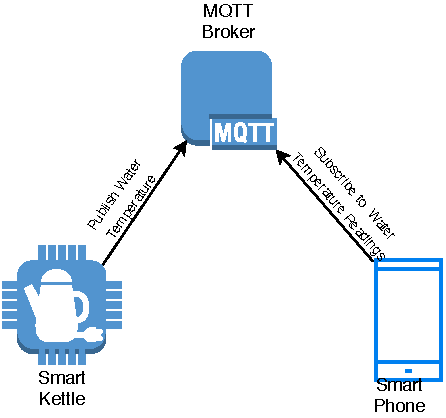
\includegraphics[width=0.5\textwidth]{mqtt_demo}
    \caption{MQTT Broker Architecture}
    \label{fig:mqtt}
\end{figure}

In short, MQTT, fully expanded to Message Queueing Telemetry Transport is an open protocol, certified by OASIS and ISO\cite{banks2019mqtt}, responsible for publisher-subscriber architecture. It's important to point out that MQTT is not a piece of software or a server, but rather a set of standards defining what potential clients can expect (what kind of responses and data) while connection to brokers following the standard. Figure \ref{fig:mqtt} briefly shows how MQTT-compatible broker can relay information between clients. Smart Phone and Smart Kettle don't have to be online at the same time in order to receive information, nor Smart Phone is even permitted to initiate direct connection to Smart Kettle. The broker's responsibility is to track connected subscribers (which must specify topic of their interest) and maintain connection until subscribe advertises session termination or abruptly disconnects (e.g. loss of power or unreliable connection).

In MQTT architecture, Client ID identifies each of the connecting entities (publisher / subscriber) and Topic identifies a bridge between publishers and subscribers connected to the same topic. For example, a Smart Kettle could be publishing temperature readings under topic called ``UK/Aberdeen/Kettle'' - then, Smart Phone would need to request the same topic to receive those readings. 

\subsubsection{\textbf{Message persistence}}
This will be discussed in depth, when I will describe the process of publishing and subscribing, but it's worth pointing out that by default, the messages are not saved nor cached on the broker. That is, if Kettle publishes the temperature reading, but there is no subscribers listening to this information, the message will perish. This is not ideal, for situation where smart device could wake up only every couple of minutes and then go to low-power mode again. To address this, MQTT Messages can be enriched by ``Retain'' flag. If such flag is present, the broker will keep the message and send it straight away to any new subscribers requesting given topic. This is also useful for issuing commands to IoT devices - for example, a phone could send command to turn off the lights with ``Retain'' flag set. Then, the smart light switch could check for retained messages every couple of minutes, removing the need of constant connection.

\subsubsection{\textbf{Implementation}}
MQTT by itself is only a collection of standards instructing implementors on what patterns should be followed and the structure of particular messages, thus it's not shipped with any piece of software. It assumes operation on TCP layer of network (although newer versions also allow for WebSocket support \citep{mijovic2016comparing}), thus also allowing for encrypted connection via Transport Layer Security. Every exchanged message is a TCP packet, following strict convection - which in case of deviation is discarded as corrupted.

Two of the implementations that I have considered during this project are Mosquitto\footnote{https://mosquitto.org/} by Eclipse and Moquette\footnote{https://github.com/moquette-io/moquette}. The former written in C and the former in Java, although there is many, many more. In a paper by \citet{de2019performance}, scientists compare Moquitto and RabbitMQ, arguining their choice by the offered cloud infrastructure with greater scalability opportunities. Moreover, there are solutions that are paid, whereas the considered approaches are free and open source allowing for better understanding of operations. The paper is concluded with the finding that hardware and network latency has a far greater impact on the performance, rather than choice of the individual broker, which leaves the decision mostly down to offered extra features.

Mosquitto also offers a Docker container \cite{light2017mosquitto} in which the broker can be run, allowing for further isolation and removal of extra dependencies.

\subsubsection{\textbf{Publishing}}

The most popular method of passing MQTT messages is still under Transport layer, as TCP packets. This allows for slightly higher freedom (compared to stricter protocols, such as HTTP), at the cost of more sophisticated parsing. MQTT standard is composed of several message types with the most important being:
\begin{itemize}
  \item CONNECT - used to initiate the connection
  \item PUBLISH - used by the client to publish messages and by the broker to publish messages to subscribers
  \item SUBSCRIBE - used by the client to request subscription to a given topic
  \item UNSUBSCRIBE - used by the client to request removal of subscription to given topics
  \item Along with relevant *ACK counterparts (e.g. CONNACK) used to indicate successful transmission of the message
\end{itemize}
As shown on figure \ref{fig:mqtt_publish}, the publishing flow starts with the CONNECT messages. Inside, there are several flags included, such as Quality of Service requested (MQTT can periodically send heartbeat ping to clients to check if they are still alive), requested version of MQTT protocol (at the moment, v5.0 and v3.1). This part is also referred as ``Variable header''. The second part, known as ``Payload'' consists of client ID.

Then, once the client has established its identity to the broker, the broker responds with CONNACK message, which contains bit informing whether further connection is allowed or not. From this point, the client is cleared to start publishing session.

Usually, for every message to be published, there is one PUBLISH packet. Newer version of MQTT allow for spreading larger messages across multiple packets, although this will not be covered in this paper. The PUBLISH packet contains mostly two properties - topic to be published on and the actual payload. Each of the properties is prepended with 8 bytes indicating the length. From this fact, we can derive the maximum possible size of individual payload - 65535 characters (pure ASCII, no Unicode, which may take more than 1 bytes per character). Same as with CONNECT, each message is responded to with PUBACK, acting as a receipt for receiving the payload.

The client can continue to publish extra messages without having to connect again, as long as the TCP session has not been terminated. Should the client want to disconnect, it should follow standard TCP flow, i.e. issue FIN/ACK packet to the broker. For situation, where the connection has been terminated abruptly, there are options such as Will flag (message to pass in case of sudden disconnection) or Keep Alive (to indicate how long should the connection be kept alive for before assuming the client has lost connection).

\begin{figure}[ht]
    \centering
    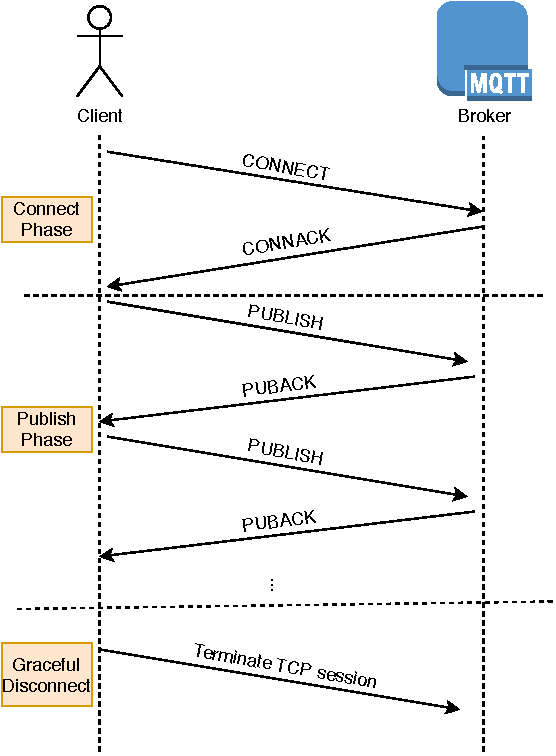
\includegraphics[width=0.6\textwidth]{mqtt_publish}
    \caption{Publishing flow with MQTT}
    \label{fig:mqtt_publish}
\end{figure}


\subsubsection{\textbf{Subscribing}}

Subscribing flow is quite similar to Publishing, with some minor differences. Following figure \ref{fig:mqtt_subscribe}, first and foremost a connection needs to be established by instating standard TCP/TLS session and then sending CONNECT packet. The contents follow the same standard, i.e. containing information such as Client ID or even optional parameters in a form of ``key: value'' (particularly useful for this project).

\begin{figure}[ht]
    \centering
    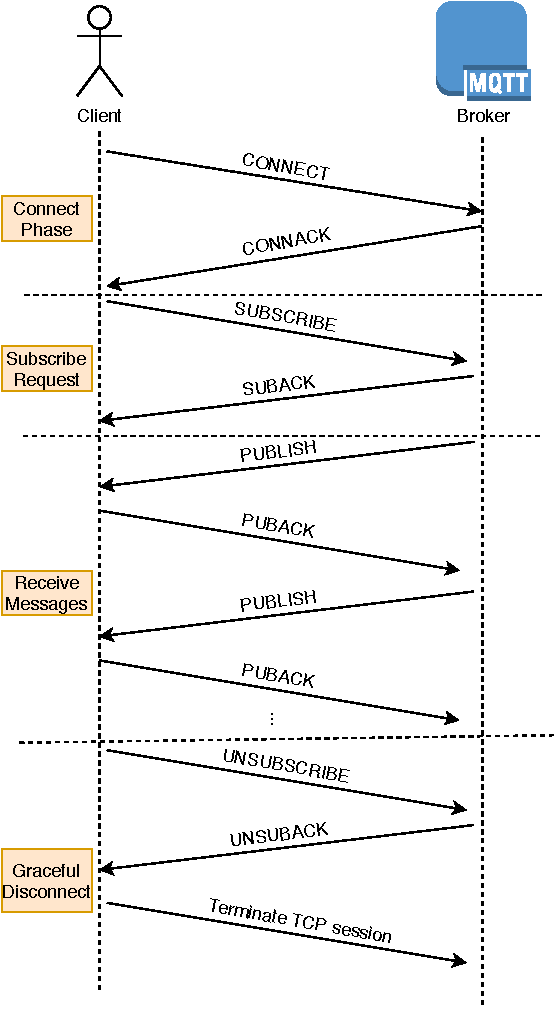
\includegraphics[width=0.6\textwidth]{mqtt_subscribe}
    \caption{Subscribing flow with MQTT}
    \label{fig:mqtt_subscribe}
\end{figure}

After successful connection, Client can proceed to send request for subscription. Similar with PUBLISH packet, client specifies type of the packet in the variable header and then requested topic for subscription in the payload. The extra element is the QOS flag - Quality of Service. MQTT has 3 levels of QOS:
\begin{enumerate}
  \item 0 - No response to PUBLISH messages
  \item 1 - PUBLISH messages will be followed by PUBACK
  \item 2 - More granular control over PUBLISH, with extra packets such as PUBREC (Publish Received), PUBREL (Publish Release) and PUBCOMP (Publish Complete).
\end{enumerate}

Once the SUBSCRIBE message has been processed and approved by the broker, it will issue SUBACK message and remain connect to the client. From this point, any message that is published on the topic specified in SUBSCRIBE packet will be published (as PUBLISH packet) to every client currently subscribed to it. Of course, depending on requested QOS, the broker might then await for PUBACK message (or even issue extra messages such as PUBREC, PUBREL, PUBCOM). The diagram demonstrates a simple exchange with QOS set to 1. 

\begin{table}[h]
\centering
\begin{tabular}{lllllllllllllll}
\cline{1-14}
\multicolumn{1}{|l|}{82} & \multicolumn{1}{l|}{0C} & \multicolumn{1}{l|}{00} & \multicolumn{1}{l|}{01} & \multicolumn{1}{l|}{00} & \multicolumn{1}{l|}{07} & \multicolumn{1}{l|}{F} & \multicolumn{1}{l|}{L} & \multicolumn{1}{l|}{Y} & \multicolumn{1}{l|}{T} & \multicolumn{1}{l|}{R} & \multicolumn{1}{l|}{A} & \multicolumn{1}{l|}{P} & \multicolumn{1}{l|}{00} &  \\ \cline{1-14}
1                        & 2                       & 3                       & 4                       & 5                       & 6                       & 7                      & 8                      & 9                      & 10                     & 11                     & 12                     & 13                     & 14                      &  \\
                         &                         &                         &                         &                         &                         &                        &                        &                        &                        &                        &                        &                        &                         &  \\
                         &                         &                         &                         &                         &                         &                        &                        &                        &                        &                        &                        &                        &                         & 
\end{tabular}
\caption{Example SUBSCRIBE to topic FlyTrap packet}
\label{tab:sub_packet}
\end{table}

To close off MQTT, I also wanted to overview an example packet and dissect it byte by byte to demonstrate exactly what kind of information is included - this can be seen in table \ref{tab:sub_packet}
\begin{enumerate}
  \item [1] Control field, specifies type of the message (CONNECT, SUBSCRIBE etc.)
  \item [2] Remaining length of the message. Can be expanded to 2 bytes.
  \item [3-4] Packet ID
  \item [5-6] Payload length
  \item [7-13] Payload. Corresponding hex encoding of characters, replaced with actual characters for clarity
  \item [14] Requested QOS
\end{enumerate}


\section{Related Work}
This section will talk about other scientific papers which had similar goal in mind, by combining  blockchain technologies with IoT or even MQTT brokers.


\chapter{Requirements \& Architecture}
\section{Requirements}

\subsection{Function Requirements}

\subsection{Non-function Requirements}

\subsection{Use-cases}

\section{Architecture}

\chapter{Design\label{chap:design}}
In this chapter, I will talk in depth the elements that I created during this project and how they inter-connect. You can expect a design charts showcasing high-level overview, alongside dividing it onto smaller subsections - each independent and capable of running on its own. I will also provide explanation on novel approaches such as verifying the authenticity of the connecting clients, data model stored on blockchain or how the connection is secured from man-in-the-middle attacks through TLS encryption.

\section{Architecture}
This section includes the diagram of them system and two sample workflows demonstrating how packets are flowing through the framework.
\subsection{Overview}
\begin{figure}[h]
    \centering
    \makebox[\textwidth][c]{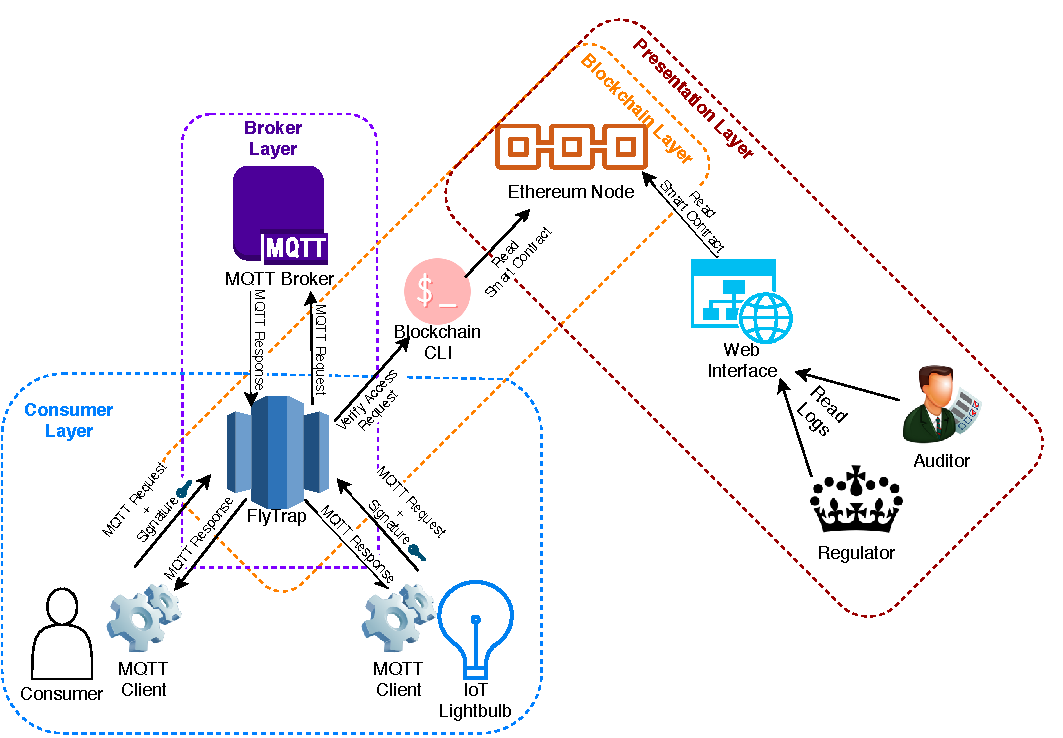
\includegraphics[width=1.2\textwidth]{flytrap}}
    \caption{FlyTrap high-level architecture overview}
    \label{fig:flytrap}
\end{figure}
Figure \ref{fig:flytrap} presents an overview of the system, decomposing it onto four layers, each responsible for different part of the framework. It also demonstrates how those layers are coupled and the direction of data flowing between them.

To overview, we can distinguish four layers:
\begin{description}
    \item[Consumer Layer] - layer responsible for interacting with end-devices. To them, FlyTrap should be indistinguishable from normal MQTT broker and thus accepts/responds with MQTT v5.0 compliant TCP/TLS packets. In order to compute the signature and attach it to 
    \item[Consumer Layer] - layer where FlyTrap acts like a client for MQTT Broker. Similar to Consumer Layer, all packets sent by FlyTrap need to be compliant with MQTT standard in order to receive valid responses from the broker. In this situation, used MQTT broker is not relevant - as long as it implements the standard.
    \item[Blockchain Layer] - layer in which FlyTrap performs communication with Ethereum node through a separate CLI. FlyTrap is capable of either reading the past contracts/transcations or submitting new ones. That's also the only way to amend the state of the blockchain - given the master private key has remained secret.
    \item[Presentation Layer] - layer used by FlyTrap's endusers which allows to overview the state of the blockchain in a user-friendly way, easily extracting most relevant information such as recent access changes or audit trail for major operations on the chain.
\end{description}


\subsection{Sample successful PUBLISH workflow}
To provide further context, figure \ref{fig:workflow_success} provides an example process in which a client wants to publish a message to the broker and is successful in doing so. The diagram shows step-by-step logic performed at each stage of the connection, until client receives the response. I'll annotate each step with either \textbf{BL} - Blockchain Layer, \textbf{CL} - Consumer Layer or \textbf{ML} - MQTT Broker Layer to signify on which layer this step is taking place on.
\begin{figure}[h]
    \centering
    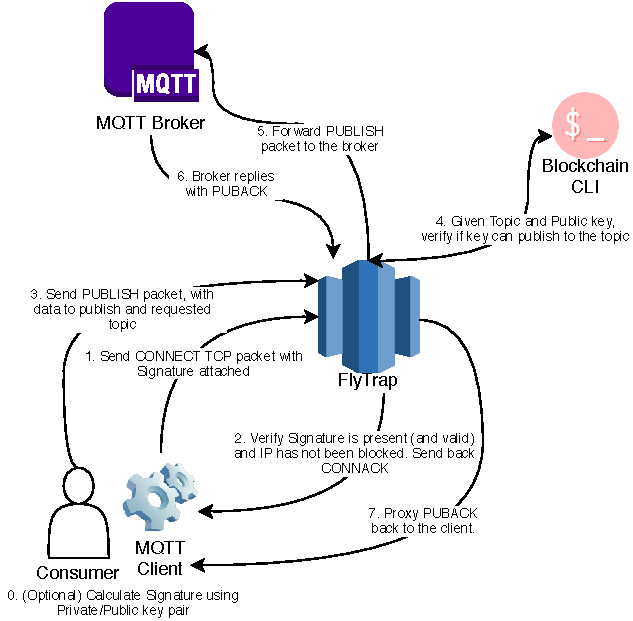
\includegraphics[width=0.8\textwidth]{workflow_success}
    \caption{Example successful workflow to publish a message on the broker through FlyTrap}
    \label{fig:workflow_success}
\end{figure}

Explanation of each step:
\begin{enumerate}\addtocounter{enumi}{-1}
    \item Marked as optional, since each Client can accept pre-computed signature, which can be loaded onto the device; this can be helpful for situations where there is not enough computational power for calculations. (\textbf{CL})
    \item Client sends CONNECT packet, including signature + public key in the optional fields of MQTT message. (\textbf{CL})
    \item FlyTrap will extract the signature from the optional field and then verify its integrity. It will also check if the client has not been attempting many unsuccessful connections. Finally, FlyTrap will repond with CONNACK, signaling to the client that it may now submit relevant payload packets. If the integrity check has failed, CONNACK would also have a flipped flag indicating rejected connection and cease further communication. (\textbf{CL})
    \item Client will now forward the relevant PUBLISH/SUBSCRIBE packet to FlyTrap (as it still believes that it's a regular MQTT broker). (\textbf{CL})
    \item FlyTrap will now extract requeste topic from the MQTT packet and communicate with the Blockchain, presenting Public Key and requested topic to verify whether data can be accessed. For this example, the access check was successful. (\textbf{BL})
    \item FlyTrap proxies (unchanged) PUBLISH packet to the actual MQTT broker. (\textbf{ML})
    \item MQTT broker will now respond with PUBACK, indicating successful PUBLISH. (\textbf{ML})
    \item Finally, FlyTrap will proxy the same PUBACK packet back to the initial client to let them know that the operation was successful - and at the end, gracefully terminate the connection. (\textbf{CL})
\end{enumerate}

\subsection{Sample failed PUBLISH workflow}
Operation similar as in the previous section with the difference being that this time connection is not allowed, as the presented Public Key is not allowed to publish information on the given topic. For the brevity sake, I will skip explaining steps 0-3 - as they are identical as with the successful scenario. I will also use the same notation to signify which layer is responsible for this operation.

\begin{enumerate}\addtocounter{enumi}{4}
    \item Having verified authenticity of Public Key, FlyTrap again tries to verify with the Smart Contract whether the client can access the topic. This time though, the reponse is negative and the client is not allowed to publish on the requested topic.
    \item FlyTrap will send PUBACK back to the client, setting reason code\footnote{https://docs.oasis-open.org/mqtt/mqtt/v5.0/os/mqtt-v5.0-os.html\#\_Toc3901124} to "Not authorized", at the same time terminating the connection with the client. To client, the situation is identical as with providing invalid username/password for a vanilla MQTT broker.
    \item Framework will verify with the cached values to check if the originating IP has not exceeded maximum number of allowed tries. If it did, it can place it on a blacklist and every subsequent connection will be denied for the specified time. In this example, that's 5 minutes. This step is optional
    \item If the ban happens, FlyTrap will also register a new transaction on the blockchain to persistently log this event for the purposes of checking potential attack spikes or generating reports w.r.t.  captured data. This step is also optional, as it depends on the previous one.
\end{enumerate}

Note: as you can see, the MQTT Broker is never connected to nor contacted with the potentially malicious message. FlyTrap rejects the message and forbids the connection. 
\begin{figure}[h]
    \centering
    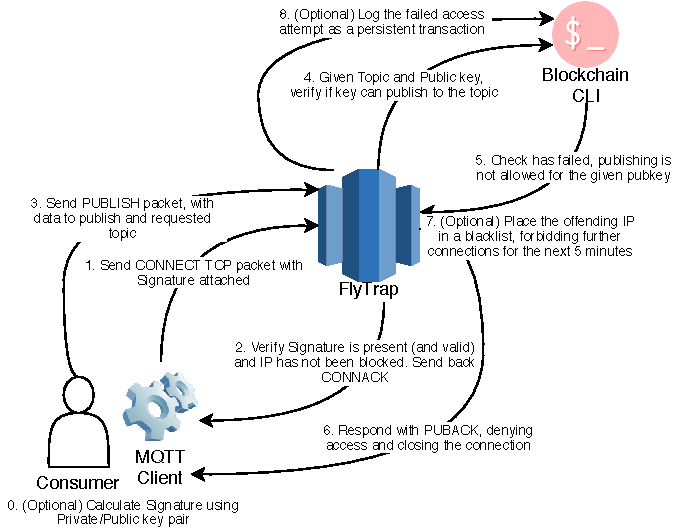
\includegraphics[width=0.9\textwidth]{workflow_fail}
    \caption{Example failed workflow to publish a message on the broker through FlyTrap}
    \label{fig:workflow_fail}
\end{figure}

\section{Consumer Layer}
First and foremost, the consumer layer. This part of the framework handles all connections between clients attempting to PUBLISH or SUBSCRIBE to data. To them, FlyTrap should be indistinguishable from a vanilla MQTT broker, which should be accepting all regular MQTT payloads. Though since every MQTT client produced in this project can connect with every MQTT Broker, a specific client is required for connection with FlyTrap - which is further explained in the section below. Moreover, an approach of identifing whether the client holds a Private Key for the presented Public Key is also needed and explained. 
\subsection{MQTT Client}
As mentioned above, FlyTrap makes use of the introduced in MQTT v5.0 User Properties\footnote{https://docs.oasis-open.org/mqtt/mqtt/v5.0/os/mqtt-v5.0-os.html\#\_Toc3901068}, allowing clients to include key-value pairs in the MQTT packets, which then can be utilised by the brokers (or other middleware). That's also where the signature and public key is being placed by the client when attempting connection with FlyTrap - and that's also the need for a custom client, since normal clients are not capable of producing highly specilised signatures for the purposes of connecting with Ethereum blockchain.

It is important to point out, the client is only slightly altered to provide (and compute if needed) the signature from public/private key pair. It is not a crucial system of the framework, as any client capable of setting User Properties for MQTT message would be sufficient, though for the purposes of this dissertation, custom implementation has also been designed and included.
\subsection{Secure Proxy}
In order to enable FlyTrap to make decisions on whether the requests for publishing or subscribing should be accepted or denied, a secure proxy needs to be established between the clients and the MQTT Broker. As the communication between the broker and the consumers happens on Transport Layer, it is possible to insert a middleman who would be capable of inspecting the packets flowing through, dissecting it for relevant information and finally make a decision about their future journey - all without the client ever knowing that someone has intercepted the connection. 
\begin{figure}[h]
    \centering
    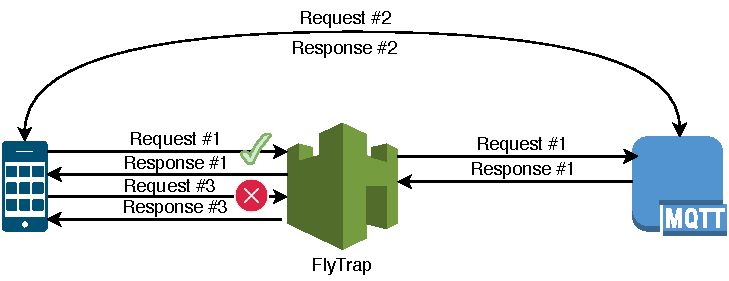
\includegraphics[width=0.8\textwidth]{tls}
    \caption{FlyTrap acting as a proxy}
    \label{fig:tls}
\end{figure}
Figure \ref{fig:tls} demonstrates all 3 possibilities when client attempts connection to a broker. In the Request \#1, FlyTrap will dissect the packet and confirm that the phone indeed can be allowed to access specific topic and then start bidirectional proxy with the broker, passing the TCP packets between two. Request \#2 shows that the same packet can be used for vanilla MQTT Broker without FlyTrap, thus decoupling the client and secure proxy, as the former can be used without the need to change the latter. Finally, for the third request, it is found that the client cannot access the requested resource and will be presented with CONACK response, with access denied flag set, terminating the connection. Though, in order to make such decisions, the proxy needs to inspect the contents of the packets.

Although this solution enough will not be sufficient, as quickly as FlyTrap can tap into the connection, the same can be assumed for potential malicious actors, which could be listening on the flowing through packets. The solution will support an extension to standard TCP - Transport Layer Security, or TLS for short, responsible for encrypting the TCP packets, significantly reducing the threat of man-in-the-middle attacks.

TLS sessions can be summarised in the following steps:
\begin{enumerate}
\item Initiate standard TCP session
\item ClientHello with client's cypher capabilities 
\item ServerHello and exchange of the cypher suite, along with server's certificate
\item Key exchange and change of cypher spec
\item Encrypted session starts
\end{enumerate}

It's important to point out, that due to step 3 requiring server's certificate, FlyTrap will need to either obtain a copy of broker's certificates or generate a new pair, ensuring that the connecting clients will trust it. Though, secure TLS connection remains optional, as it is understandable that sometimes enhanced security might cause undesirable performance losses or the MQTT broker simply doesn't support TLS connections - TLS will be configurable via command line arguments.

For every new connection, a new thread (or, go routine) is spawned which has its own context and is separated from others.

\subsection{Authenticity of public keys}
Public Keys from the Ethereum wallet are used as an identifier when determining whether client can access given resource or not. Though it only handles a part of the problem. Public Keys, by definition, are public, meaning that anyone could impersonate legitimate holders of the public/private key. This calls for an approach similar to the Certificate Authority problem when attempting encrypted HTTPS connections. Unfortunately, FlyTrap cannot expect every IoT device to have its own set of certificates, which would then need to be trusted by the framework in order to become recognisable - as those devices are often of limited storage and power.

To solve the problem of establishing whether the person presenting a public key also holds a corresponding key, signatures are used. Below you can see two figures, each outlining client side and FlyTrap side of the signing/verification process.

\begin{figure}[h]
    \centering
    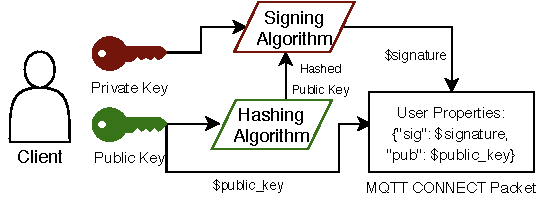
\includegraphics[width=0.8\textwidth]{sign}
    \caption{Client signing Public Key and attaching it to the message}
    \label{fig:sign}
\end{figure}

Figure \ref{fig:sign} shows how client - in possession of public/private key pair produces a signature which then is attached to the final MQTT CONNECT packet. First, it hashes the public key using Keccak-256 algorithm \cite{bertoni2009keccak} (commonly used in Ethereum, e.g. for block hashes), then it uses the private key to sign this hash and attaches obtained signature to the user properties part of the MQTT CONNECT message. Plain-text version of the public key is also attached in another field. Ethereum signatures are created by signing arbirtary bytes through generated private key - which then can only be verified using the corresponding public key. It is also possible to extract signed bytes from the same signature in the process.

\begin{figure}[h]
    \centering
     \makebox[\textwidth][c]{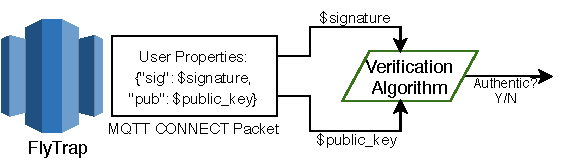
\includegraphics[width=1.1\textwidth]{verify}}
    \caption{FlyTrap verifying the signature}
    \label{fig:verify}
\end{figure}

Then, as per figure \ref{fig:verify}, FlyTrap receives the CONNECT packet and extracts both the signature \& public key from the message. As the corresponding private key for the public key was used to produce the signature, framework verifies this through Verification Algorithm. The output is a binary yes/no value - determining whether the public key was used to create the signature - along with the signed value (in this case, hashed public key) by the client. Then, framework can verify whether both signature was indeed created with the private key corresponding to the attached public key and (by hashing it again) compare the extracted value with the attached public key. This gives a definite answer that the person presenting the public key also holds the private key and thus is successfully authenticated.

For Ethereum, both Verification Algorithm and Signing Algorithm is part of Elliptic Curve Digital Signature Algorithm \citep{johnson2001elliptic}, where public key has exactly 160 bits (which, coincidentally, is also used for ETH addresses). Hashing Algorithm - as mentioned above - is Keccak-256.
\subsection{Protecting from brute-force attacks}
Some of the failed attempts can result in persistent log to blockchain, which often implicates costs - especially if FlyTrap is operating on a public blockchain. This can open a door for malicious actors attempting to drain the framework from available funds by logging a lot of operations in a short span of time. Distributed Denial of Service (DDoS) attacks can also occur and overload the server, which - depending on hardware - could only handle a limited number of simultaneous connections.

To combat those problems, framework will track any failed authentication attempts in an internal dictionary, mapping IP address to the number of failed attempts. This dictionary then will be consulted whenever a new connection is initiated. If it is, then the TCP link will be shut down and client informed that it is currently blacklisted. Though to give benefit of a doubt, there is a grace period of 2 prior failed attempts before a timed ban is applied. Whenever failed authentication occurs, the counter is increased by one - and if that count increases 3, the connection is terminated and dictionary updated with time 5 minutes in the future - that's the earliest time given IP can attempt connection again.
\section{Broker Layer}

This layer is where the communication with the actual MQTT Broker occurs. Normally, it would be desirable to place both FlyTrap and the broker (e.g. Mosquitto) on the same machine (or at least the same network) to minimise the latency - though it's not necessary. Depending on the outcome of the authorisation from the Client Layer, every packet from the client is forwarded to the broker and every packet from the broker sent back to the client. Since each connection is an individual thread, it also maintains information such as originating (\& destination) address and port - and this information will persist as long as the original connection Client <=> FlyTrap remains open - which will only be terminated if client times out, requests disconnection or for any reason authentication to FlyTrap fails.

Similar to the section discussing encrypted connection, FlyTrap is capable of either connecting with TLS-capable brokers or via plain TCP if desired (though keeping the security implications in mind, as everyone intercepting the connection would be able to read the payload).

\section{Blockchain Layer}
In this layer, communication with the Ethereum node occurs. As described in architecture section, FlyTrap can either read or write new data onto the chain. FlyTrap should be allocated its own smart contract containing chain code capable of verifying connecting clients and relevant data structures. 
\subsection{Data model}
The root of all communication with blockchain is a smart contract that contains all chaincode responsible for retrieving and storing information required by FlyTrap. Each organisation or entity willing to use FlyTrap should configure and deploy a new contract, which would be tied to a singular owner (i.e., a private key). Ethereum's chaincode execution can be limited to only particular set of addresses, here most of the sensitive operations (such as addining new publishers or subscribers) are restricted to either an owner or payable ETH (set by the owner) - if the requestor is not an owner.

Then, each contract contains a singular variable called ``topics'' which is a mapping (dictionary structure in Solidity, programming language for ETH) from string (name of the topic) to structure ``Topic'' where the metadata can be located, such as control lists. Every person can create their own topic on the contract, of which they would become the owner - this operation can be payable, if set so by the contract's owner, meaning topic creators would need to pay a fee. Figure \ref{fig:uml_topic} shows all fields used in FlyTrap's chaincode placed on blockchain, to further explain usage and purpose of each of the fields:
\begin{figure}[h]
    \centering
    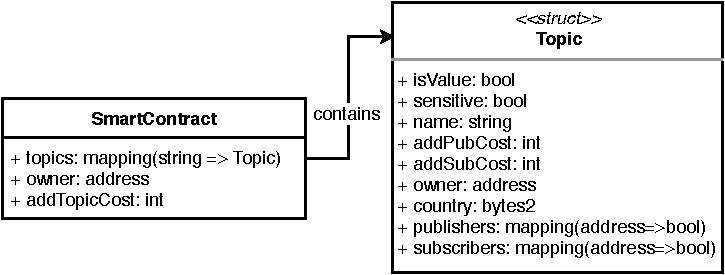
\includegraphics[width=0.9\textwidth]{uml_topic}
    \caption{Topic structure stored on Blockchain}
    \label{fig:uml_topic}
\end{figure}
\begin{description}
    \item[isValue] - in Solidity, it is not possible to determine whether given key exists in the mapping, as every value points to some arbitrary address space. An extra field helps to mitigate this issue, e.g. to avoid overwriting existing topics with new data.
    \item[sensitive] - a bool flag marking given topic as sensitive which enhances it with extra data reporting functionality outlined in section \ref{sec:reports}.
    \item[name] - a string storing topic's name, as used by the clients on the broker. It's also used as the key in the topics mapping.
    \item[addPubCost] - integer, allowing to set a price on adding new publishers to given topic. Then, the payment will be transferred to topic's owner.
    \item[addSubCost] - integer, similar as above, but for publishing.
    \item[owner] - ETH public address of the person that created this topic.
    \item[country] - 2-letter encoding of country to which access should be limited to for all subscribers/publishers.
    \item[publishers] - mapping from address of a person to a true/false bool value to determine whether given public key can publish to this topic. It's a way of creating dynamic lists in Solidity, while maintaining $O(1)$ lookup time.
    \item[subscribers] - same as above, but for subscribers.
\end{description}

Apart from base structure holding information inside the contract, events are also utilised. Event is a special structure used in Solidity, which attaches itself to the transaction log. Meaning that it is possible to append information such as user-specified reason or timestamps to all operations. This is then encoded in Application Binary Interface (ABI)\footnote{Encoding type used in Solidity: https://solidity.readthedocs.io/en/latest/abi-spec.html} JSON and sent along with the transaction. Though, it is also possible to emit empty events solely for the logging purposes \citep{dannen2017introducing}.  Figure \ref{fig:uml_event} outlines what each event consists of:
\begin{figure}[h]
    \centering
    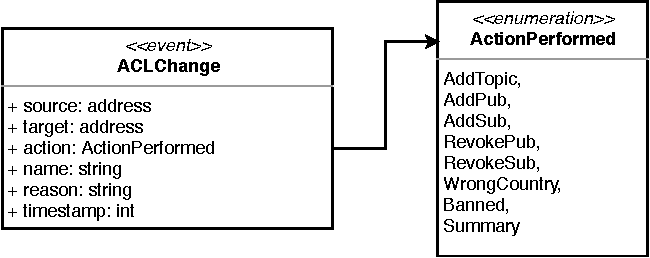
\includegraphics[width=0.8\textwidth]{uml_event}
    \caption{Event structure as stored in transaction log}
    \label{fig:uml_event}
\end{figure}

\begin{description}
    \item[source] - ETH address of the entity that caused the log to emit. E.g. for adding new topics or modifying topic's properties (such as subscribers) it's the initiators request. For system-caused logs (e.g. report summaries), it'd be contract's address.
    \item[target] - ETH address of the entity affected by the logged action. E.g. for revoking publishers/subscribers, it'd be the person that's getting removed.
    \item[action] - enumeration which defines the exact reason for the emitting the log, this can be one of the following values:
    \begin{description}
        \item[AddTopic] - when a new topic is created on the contract
        \item[AddPub] - when a new person is added as a publisher to the topic
        \item[AddSub] - when a new person is added as a subscriber to the topic
        \item[RevokePub] - when a person is removed from authorised publishers in the topic
        \item[RevokeSub] - when a person is removed from authorised subscribers in the topic
        \item[WrongCountry] - when a connection was attempted from an IP located in country that's not permitted
        \item[Banned] - when a person failed to authorise when connecting for three times in a row and was placed on a blacklist
        \item[Summary] - system generated log for sensitive topics (see \ref{sec:reports}
    \end{description}
    \item[name] - string used to signify which topic was affected. If action doesn't involve a topic, it contains offending IP address.
    \item[reason] - string provided either by the user or by the system to provide further context on the action (in particular, to answer questions given by GDPR, ``why was access provisioned?'')
    \item[timestamp] - UNIX timestamp (expressed as integer) to determine when the transaction has happened
\end{description}
\subsection{Report Generation}\label{sec:reports}
For the most sensitive topics, it is possible to enhance the security with extra measures and reporting. For every topic marked as sensitive, FlyTrap would maintain an in-memory list of all publishers or subscribers that have recently accessed the topic. Then, every specified period of time, a log will be generated and placed on blockchain that would outline all Ethereum public keys that have either published or subscribed to the given topic.

To put it in an example: if the reporting frequency is set at 30minutes and the system is started at 12:00, then client A publishes to topic  X at 12:05 and client B publishes to topic X at 12:15, finally at 12:30 a report would be generated and placed on blockchain which would signify that both client A \& client B published to topic X between 12:00 and 12:30. The reports should be read as follows: In the past X minutes, following public keys accessed following sensitive topics. 

It is important to consider the implications of more and less frequent reporting - since every transaction placed on a blockchain with PoW consensus algorithm has embedded gas price\footnote{Gas is a unit of work performed on Ethereum. The more complex the operation, the more gas is required and thus more ETH currency is needed}, so the owner of the system would need to either accept the increased costs or decrease the reporting frequency. Of course, for PoA algorithms, there is not gas cost, but still chaincode's size would grow faster in case of more frequent reportings. But with decreased frequency, the precision also falls, so if our reporting is set to 24hrs, now we can only determine the access history in daily windows (rather than 30min ones, as shown in the example above).
\subsection{Caching operations}
Communicating with Blockchain is a computationally expensive operation and it is vital to ensure that it happens as rarely as possible in order to limit the latency caused by the security checks. Following brute force approach, framework would issue a new request every time a connection starts - regardless whether it is part of a series of requests arriving in bulk. FlyTrap is using Ethereum as a de facto database layer, but at the same time aiming to cache the operations in-memory, which can be then quickly accessed if repeated requests occur. For checking the permissions, whenever a new request is issued, the result is stored in a map with mutex lock (to avoid race conditions).

To avoid memory filling too quickly (and eventually reaching the capabilities of the server that is running the software), the mapping used for caching will be erased every 24hrs or when the process is terminated/restarted - whichever happens first.

\subsection{Interacting with blockchain}\label{sec:interact}
As FlyTrap aims to be deployed on a publicly available blockchain, anyone can interact with the data (as long as they pay the requested fee and/or identify with the relevant owner's private key). For administrative operations, a simple CLI is also included, which can be called directly (not necessarily through FlyTrap) to perform administrative tasks, such as adding new topics, modifying topics restrictions etc. 
\section{Presentation Layer}
This layer combines everything above in a front-end allowing users to inspect and interact with stored information. Similarly to section \ref{sec:interact}, this could also be read through any of the publicly available frontends used to interact with Ethereum transactions, but to provide a complete package, the project will also ship with a simple website aiming to satisfy requirements stated in chapter 3.
\subsection{Website}
The website will not allow for writing data to blockchain (thus, doesn't require Ethereum wallet) which implies that all reading operations are free. Instead of using the Blockchain CLI from Blockchain Layer, the website will ship with API of its own, which will perform calls against the specific Ethereum node directly.

\chapter{Implementation\label{chap:implementation}}
This chapter is discussing the technical specifications of the project and discuss the decisions that affected the process. I will also overview my workflow and iterative approach to the project. Last but not least, I will include and credit a list of third-party libraries that this framework makes use of.

\section{Development process}

In this section, I will outline how the work on my dissertation was conducted along with pointing out the pitfalls and making sure that the produced code remains fully functional.

\subsection{Project plan}

\begin{figure}[h]
    \centering
    \makebox[\textwidth][c]{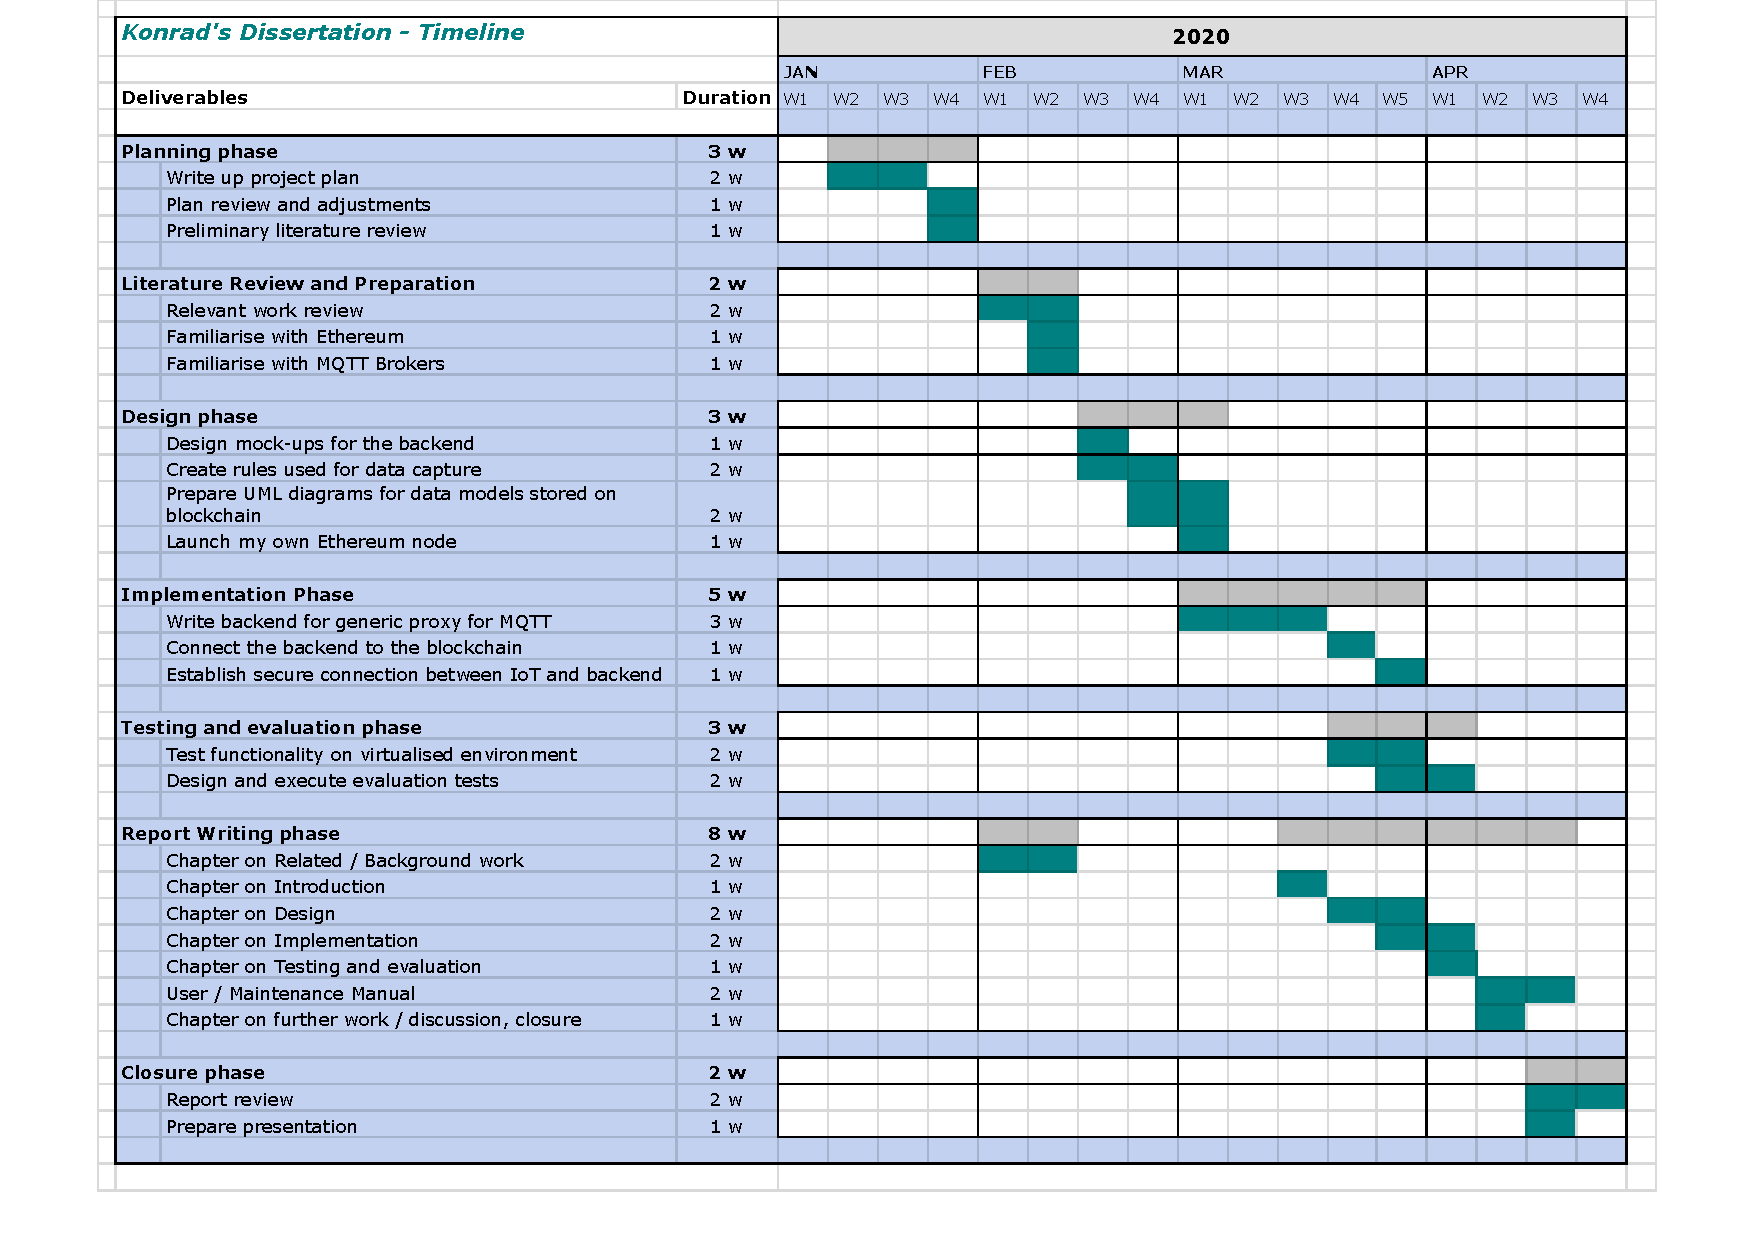
\includegraphics[width=1.1\textwidth]{timeline}}
    \caption{Project timeline}
    \label{fig:timeline}
\end{figure}

Figure \ref{fig:timeline} illustrates the timeline of the project, and all included phases. Each of those tasks was divided onto smaller subsections (not shown on the diagram), which were worked on using an agile approach, as described in the next paragraph.

\subsection{Iterative Approach}

When designing my project plan, I distributed the workload into small work chunks and features which would be implemented in an iterative manner. I was following agile methodologies, dedicating each week to a different feature, where I would go through the entire development cycle for each unit. For example, generating the reports (section 4.4.2) was first introduced during a meeting with my supervisor, where I would establish the requirements and success criteria for this particular story (following definition of stories in agile approach). Then I would spend a day or two designing the flow and functionality, followed by an extra two days implementing the designed features. At the very end, I would conduct testing and regression testing to make sure that the rest of the project still remains operational. This would be concluded with a meeting with my supervisor to reflect on the sprint and determine whether success criteria were met.

\subsection{Regression testing}

Since I was following an agile workflow when working on the project, it was essential to ensure that none of the `stories' (or, tasks) affected each other when completed. Otherwise, I could have found myself in a situation where working on the reporting of the events to the blockchain might have broken another, unrelated feature, e.g. verifying the authenticity of connecting clients. That is the reason behind keeping regression testing as a vital phase of development. I was able to achieve it through continuous, automated testing - which includes unit, integration, regression and manual testing.

\section{Technologies}

In this section, I will describe the technologies used in this project, that is, languages, frameworks, third-party libraries and different approaches when writing the code.

\subsection{Languages used}

The following programming languages have been used in this project:
\begin{itemize}
 \item \textbf{Golang} (v1.14) - main driver behind the proxy, MQTT client and for communicating with the blockchain. It has also be used in the backend for the web application.
 \item \textbf{Solidity} (v0.6.6) - language used to develop smart contracts on Ethereum.
 \item \textbf{HTML5 + CSS3 + JavaScript} - frontend stack used to create a simple website to display the contents of blockchain.
\end{itemize}

\subsubsection{Golang}
Go (short for Golang) has been introduced in 2009 by Google \cite{team2009go}. It is a language which strongly follows parallel programming paradigms, allowing the developer to make use out of all available threads and cores to maximise the performance. Multi-thread performance was exceptionally sought after in this project, as FlyTrap is expected to handle many simultaneous proxy connections. In Golang, the programmer can make use of so-called goroutines, which the runtime can dynamically either place on separate cores or run them concurrently on the same core - depending on the task.

All Ethereum frameworks (such as go-ethereum or geth, explained further in section \ref{sec:tpp}) were also designed first in Golang. By deciding to write my project in Go as well, I ensured maximum compatibility, as I was able to use the official SDK's, rather than having to rely on unofficial solutions. I also was already experienced with Golang, as I spent a year in industry at Google working on several projects in that language, which decreased the learning overhead for my dissertation.

Go in the project was used to write the backend of the webserver, CLI to communicate with the blockchain and the proxy itself which handles all incoming connections.
\subsubsection{Solidity}
Solidity \cite{dannen2017introducing} is the language used to write smart-contracts in Ethereum, so it was a necessity. Its syntax is similar to Javascript, though it is statically, strongly typed. Go-ethereum includes a utility which translates Solidity code into Golang methods, which then can be used to make calls against the blockchain. There is no API which can be used to query/create transactions and rather developers need to use official SDKs published by the Ethereum team.
\subsubsection{HTLM5 + CSS3 + JavaScript}
Since the web application serves only as a presentation and demonstration, I decided against any complex JavaScript or TypeScript frameworks and rather opted for a simple solution consisting of plain HTML + CSS and JavaScript. The web app also includes a small backend; thus, asynchronous calls are performed from the client-side towards the server to fill the content tables dynamically.
\subsubsection{Considered alternatives}
Apart from Golang, I was also considering \textbf{Python} as a main driver for the project. The majority of my projects in the past included Python, and my familiarity was sufficient to avoid any roadblocks. Though, compared to Golang, there are several problems, which would be especially prominent in this project, one of them being Global Interpreter Lock\cite{beazley2010understanding} (or GIL for short), which effectively restricts the scope of possible multithreading.

The choice was also dictated by a personal preference, as I wanted to apply the knowledge I gained over my year in industry during my final year at University. I believed that having a comparison on how a language performs in both industrial and academic environment might provide invaluable experience.
\subsection{Third party libraries \& resources}\label{sec:tpp}
Following third party resources were utilised in the project. All of them include an open-source license, allowing unrestricted, free use (fulfilling \textbf{NFR4}):
\begin{description}
  \item[ethereum/go-ethereum v1.9.10] \cite{ethereum2017official} - official Go implementation of Ethereum blockchain used as a bridge between ETH nodes and any Golang programs, allowing to perform CRUD\footnote{Create, Read, Update, Delete} operations on the blockchain.
    \item[eclipse/paho.golang v0.9.1] \cite{pahogolang} - library used to unpack MQTT packets in Golang, without having to inspect each individual byte manually. It outputs a struct containing all fields as defined by MQTT v5.0 specification.
    \item[oschwald/geoip2-golang v1.4.0] \cite{geoip2} - coupled together with GeoLite2 IP Geolocation dataset from MaxMind \cite{maxmind} is used to determine the country in which the IP is located in, without having to query external APIs. 
    \item[tabulator v4.4.3] \cite{tabulator} - JavaScript library used to create dynamic data tables, which can be asynchronously populated and filtered on the client-side.
\end{description}

\subsection{Working with MQTT}
As the project heavily relies on MQTT brokers, I had to look for a solution to simulate this environment on my machine. I had two  options, either run the broker locally or use one of the publicly available test brokers
\subsubsection{Online Broker}
Both HiveMQ\footnote{https://www.hivemq.com/} and Mosquitto\footnote{https://test.mosquitto.org/} provide free, publicly available brokers capable of both TLS and plain TCP connections. Connecting FlyTrap to a live, online broker helped me test how the system would behave in a situation where FlyTrap and the broker are not located on the same machine and whether inter-network proxy works fine.
\subsubsection{Local Broker}
For maximised performance, local broker should be used, to minimise the latency of TCP/TLS connections. For that, I have used Mosquitto 1.6.9\footnote{https://mosquitto.org/blog/2020/02/version-1-6-9-released/}. I was also able to generate a new set of certificates and RSA public/private key pair for TLS connections\footnote{through `openssl' utility}.  
\subsection{Working with Blockchain}
Ethereum was to be used as a data layer for the application. Of course, testing on the public chain was unfeasible, due to the tremendous costs involved. Fortunately, Ethereum provides an easy way to start your own network, which would behave identically as the real one (including fake credits to use) - in the end, it would be indistinguishable from the real node for the applications attempting communication. When working on the project, I considered two ways of mocking (or replicating) the blockchain and in the end, made sure to test FlyTrap in both approaches:
\subsubsection{Ganache}
Ganache\cite{lee2019testing} is a framework designed for emulating Ethereum environment. It can be thought as a sandbox environment, where you can generate any required number of dummy accounts, preloaded with currency, which then can be used to transact with each other - all running on localhost, without the need of configuring a proper blockchain network. Extra blocks are mined automatically - as needed. It is also possible to dump the workspace into a file and check into version control.

Figure \ref{fig:ganache} shows how the user interface looks like. You can generate as many wallets as possible, each with public/private key pair and preloaded with 100 ETH.
\begin{figure}[h]
    \centering
    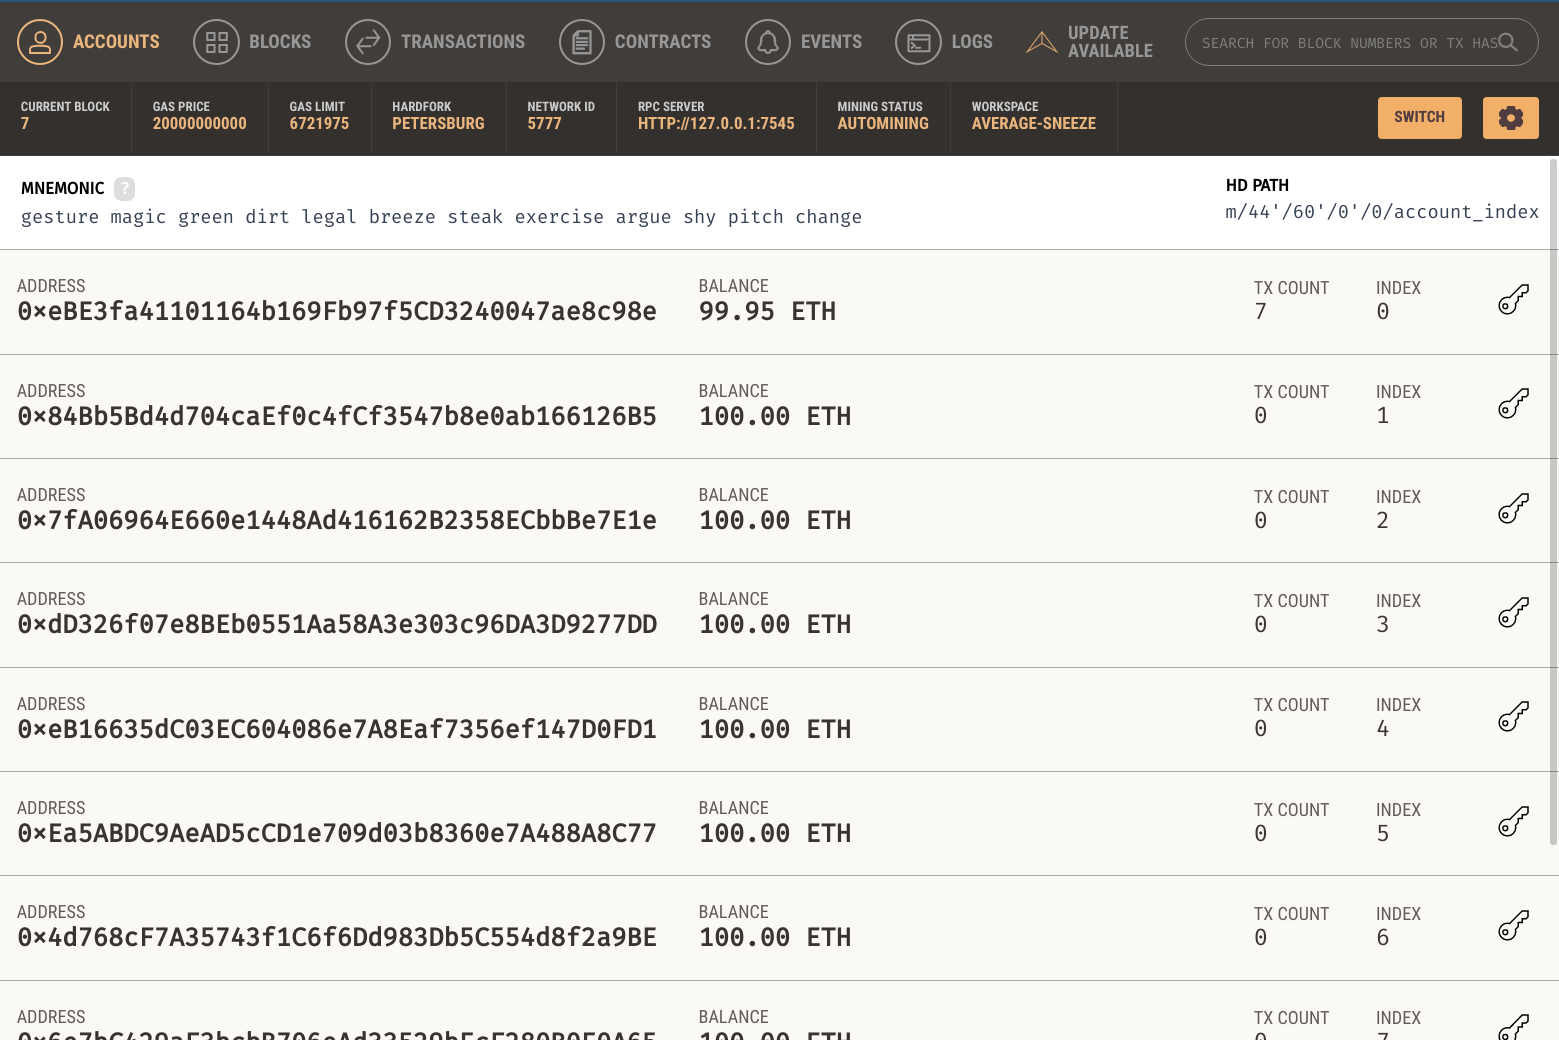
\includegraphics[width=0.9\textwidth]{ganache}
    \caption{Ganache Interface}
    \label{fig:ganache}
\end{figure}

\subsubsection{Geth}
Geth is an environment much closer to the real Ethereum node. In fact, it is used in many production environments to connect to Ethereum networks. Geth is also used in production environments to set up new networks or nodes. When testing my framework, I have set up a new Proof-of-Authority network, with only one node. Since I am in control of the network, I can configure all parameters, such as cost of gas (decreasing it down to 0), allowed accounts or speed of mining new blocks. This network is also indistinguishable from a public one, similar to Ganache. Geth can also be used to connect to live networks and start mining cryptocurrency on your workstation.
%\subsection{Development tools}
%\hl{optional, get back here if i still have some wordcount left}
%\subsubsection{Version Control}
%\subsubsection{Text Editor}

\subsection{Configuration}
Application involves a lot of configurable values, to ensure that the end-user finds their preferred combination of settings (such as TLS certs, ports - see User Manual for an overview of all possibilities). There are several ways to state constants and parameters when running any of the components:
\begin{itemize}
    \item Command line parameters - to specify the environment when running the binaries.
    \item Environmental Variables - alternative to command line parameters. FlyTrap will first inspect command line parameters and if not, will look for environmental variables defined by the host OS.
    \item Constants in the code - for some immutable values, that do not require intervention (though the option to change them remains documented).
    \item Website requests - for the web application that ships alongside the project, user can also specify fields such as contract address or which port Ethereum node is running under.
    \item Static files at projects root - since FlyTrap requires some user-provided files (such as private keys or certificates), running the proxy will require providing a path to those files via one of the methods specified above.
\end{itemize}
\subsection{Logging}
All significant operations on FlyTrap, Blockchain CLI and Web Backend are logged to standard error through log Golang module\footnote{https://golang.org/pkg/log/}. These logs are only produced for primary operations such as new connection or any actions resulting in writing to the blockchain.

They are not persistent and will disappear upon restart. Users are free to implement their own redirection to local files if desired.


% \chapter{Evaluation}\label{chap:evaluation}
FlyTrap imposes an overhead to vanilla MQTT brokers. It is vital to ensure that added layer of security does not severely impact operation of the broker, as MQTT is a time-sensitive protocol, requiring frequent and rapid responses. In this chapter, I will design experiments to measure latency caused by FlyTrap, operation cost on public blockchain and reflect back to requirements (\& user stories) to ensure that FlyTrap fulfills all of the specified needs. In the end, I will reflect on my findings and answer the stated research questions, determining my projects feasibility.

\section{Experimental design}
This section will include details on how the experiments were designed, what were the main motivations behind each of them along with the description of hardware \& software used, to ensure easy reproducibility.
\subsection{Research question(s)}
I will be looking at evaluating four separate aspects of the implementation and thus can form four research questions, which each of the subsequent sections will attempt to answer:
\begin{enumerate}
  \item How significant is the performance hit by proxing the connection through FlyTrap, as opposed to directly connecting to the broker (further referred as state-of-the-art)?
  \item How does FlyTrap's proxy scale as number of concurrent connections goes up?
  \item How expensive would be operation of FlyTrap on Proof-of-Stake type of blockchain network?
  \item Does the software fulfil specified requirements?
\end{enumerate}
\subsection{Experiments}
Each of the questions specified above will have its own designated test.

\subsubsection{Latency Evaluation} To test the performance impact, I will run the same MQTT client that was written for the purposes of this project. For first test pointing at the MQTT broker and in the other pointing at FlyTrap, which would then proxy the connection (granted access is allowed) to the broker. To capture exact response time, I will measure time taken between sending initial CONNECT/SUBSCRIBE/PUBLISH packet until a relevant *ACK response is received. Every time a new measurements is taken, FlyTrap is restarted and thus erasing all in-memory cache. For the fourth measurement, FlyTrap will not be restarted (further referred as ``Flytrap-Cached'') to take into account performance gains caused by caching. Everything will also be repeated with TLS both enabled and disabled to measure the impact of having to encrypt/decrypt TLS packets twice.
\subsubsection{Scalability Evaluation}
Latency evaluation would not be sufficient on its own to confirm FlyTrap's usability. It could be the case that singular client publishing messages is handled almost with no time loss, but as the number of clients increases (which is common for MQTT brokers to handle lot of clients at once), the response time might be growing exponentially and thus software being unusable for commercial purposes. 

Adding onto latency evaluation, I will also look at how FlyTrap performs with many simultaneous connections. 100/1000/10000 clients (where number of concurrent clients is the experiment's independent variable and average response time is the dependent variable) sending a single PUBLISH packet (with the same size for every client) will be initiated and their response times captured. Then response time for each test will be averaged and placed on a chart to determine the growth speed.  
\subsubsection{Cost Evaluation}
To test the cost, Ganache testing network will be used, as it accurately simulates real Ethereum networks. Different operations performed by FlyTrap will be considered as independent variables:
\begin{enumerate}
  \item Creating a new contract
  \item Creating a new topic
  \item Adding a new publisher/subscriber
  \item Revoking a publisher/subscriber
\end{enumerate}
As the gas cost can vary, each of those operations will be executed 100 times saving their cost in Gas (as reported by Ganache), every time using a fresh blockchain instance. Then, those prices (which would be the dependent variable) will be averaged and translated into USD for a clearer overview.
\subsubsection{Scenarios Evaluation}
Finally, to test the requirements satisfaction, scenarios described in chapter 3 of this dissertation will be used. A walk-through of the process will be included to pinpoint the benefits provided by the produced software and show how the problem presented by the use-case has been addressed..

\subsection{Testing environment}
Tests were performed on the University-provided hardware, with the specs as below:
\subsubsection{Hardware}
For tests, virtual machine provided by the University has been used. Throughout the test, the current activity on the machine was monitored through `top' utility to ensure that no other program might influence the response times. Additionally, to avoid potential slowdowns with caching, each test will have 5 warm-up requests, which will be discarded from the evaluation, followed by experimental measurements.

Table \ref{tab:hw} shows full specification of the hardware used for running the tests:
\begin{table}[h]
\centering
\begin{tabular}{|l|l|}
\hline
\textbf{Component} & \textbf{Value}                   \\ \hline
OS                 & Ubuntu 16.04.6 LTS               \\ \hline
Kernel             & 4.4.0-166                        \\ \hline
CPU                & Intel Xeon CPU E5-2630 @ 2.30GHz \\ \hline
Cores              & 4                                \\ \hline
L3 Cache           & 15 MB                            \\ \hline
RAM                & 70 GB                            \\ \hline
\end{tabular}
\caption{Hardware of the testing environment}
\label{tab:hw}
\end{table}
\subsubsection{Software}
As network latency can be unpredictable and varied, all required software and frameworks have been locally installed in the machine, with FlyTrap communicating via local TCP ports. This also includes local instances for both MQTT broker and Ethereum node. For TLS encryption, self-signed certificate was also created and provided for FlyTrap. In table \ref{tab:sw} you can find a list of specific software used for tests:

\begin{table}[h]
\centering
\begin{tabular}{|l|l|}
\hline
\textbf{Software} & \textbf{Version / Implementation}                                        \\ \hline
Blockchain        & Local instance of Geth 1.9.13 running blockchain with Proof-of-Authority \\ \hline
Golang            & Golang 1.13                                                              \\ \hline
MQTT Broker       & Local instance of Mosquitto 1.6.9                                        \\ \hline
\end{tabular}
\caption{Software of the testing environment}
\label{tab:sw}
\end{table}

All source code from the project was compiled into binaries before execution to further reduce potential noise.

\section{Latency Evaluation}
For this test we will be looking at comparing FlyTrap's performance against state-of-the-art, which in this situation would be plain MQTT Broker offering authentication through username/password. This test will provide two separate sets of results, each executed on a connection with either TLS enabled or disabled.

Furthermore, as mentioned above, each packet was submitted 105 times, discarding the first 5 results. Then for each scenario, average is calculated and placed on a bar chart. Additionally, to ensure statistical significance a two-tailed t-test has been performed on CONNECT tests to extract p-value. For SUBSCRIBE/PUBLISH - as we are dealing with three data groups - Kruskal-Wallis Test (since data is not of a Gaussian distribution, thus cannot use One-Way ANOVA Test) has been used to determine whether null hypothesis can be rejected.

Note: as no caching occurs during CONNECT stage, ``FlyTrap - Cached'' has been omitted, as it produces the same results as regular `FlyTrap'

\subsection{With TLS}
Figure \ref{fig:latency_tls} shows the average response time for each of the packets. Standard error has been omitted from the representation, as for each of the scenarios, it was found to be less than $0.01\%$. When sending the request through FlyTrap, we can notice an increase in response time of $53.73\%/61.92\%/62.67\%$ respectively for CONNECT/SUBSCRIBE/PUBLISH packets.

For FlyTrap - Cached, when compared with Vanilla, this increase is significantly less prominent, showing an increase of $18.12\%/22.19\%$ respectively for SUBSCRIBE/PUBLISH packets. 
\begin{figure}[h]
    \centering
    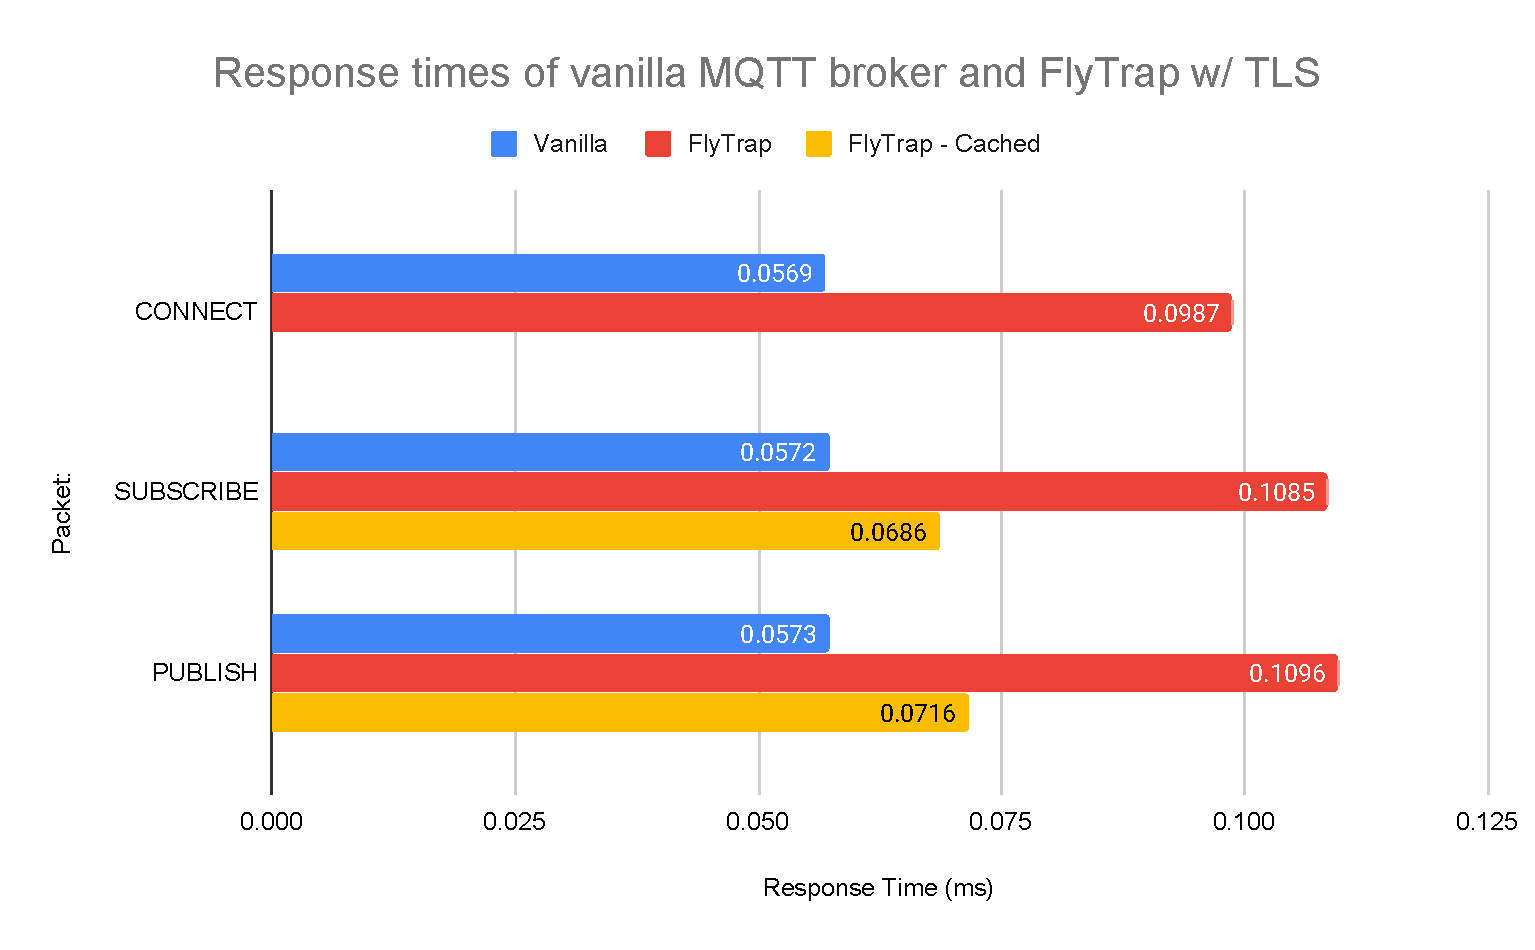
\includegraphics[width=\textwidth]{latency_tls}
    \caption{Response times of most common MQTT requests connection with SSL/TLS encryption}
    \label{fig:latency_tls}
\end{figure}

Statistical tests have been performed on all three datasets. Each of the 100 results for every packet has been compared with the counterpart, for example 100 CONNECT reponse times via Vanilla Broker vs 100 CONNECT reponse times via FlyTrap. This allows us to reject the null hypothesis, as for first test the \textit{p-value} is $<0.05$. Tests number 2.\ and 3.\ resulted with \textit{p-value} $=0$, which can be interpreted as significantly lower than 0.001.

\begin{table}[h]
\centering
\begin{tabular}{|l|l|l|l|}
\hline
\textbf{\#} & \textbf{Test Data}                       & \textbf{Performed Test} & \textbf{p-value}                      \\ \hline
1           & CONNECT: Vanilla vs FlyTrap              & Two Tailed T-Test       & $2.16*10^{-69}$                    \\ \hline
2           & SUBSCRIBE: Vanilla vs FlyTrap vs Cached & Kruskal-Wallis          & $<<< 0.001$ \\ \hline
3           & PUBLISH: Vanilla vs FlyTrap vs Cached & Kruskal-Wallis          & $<<< 0.001$ \\ \hline
\end{tabular}
\caption{Outcome of statistical tests on each the MQTT packets considered for TLS-encrypted connection}
\label{tab:ttest-tls}
\end{table}
\subsection{Plain TCP}

Test above has been repeated, this time disabling TLS encryption for both ends of the connection. First thing that we can notice is the overall decrease of response times, when compared with TLS connection. This is a clear indicator that TLS indeed adds an overhead to standard TCP connections. Experiment results were placed on a barchart in a similar manner as before. Again, standard error bars were omitted, as they were found to be less than $0.01\%$.

Figure \ref{fig:latency_notls} shows the average response time for each of the packets. When sending the request through FlyTrap, we notice an increase in response time of $18.13\%/43.30\%/31.58\%$ respectively for CONNECT/SUBSCRIBE/PUBLISH packets. For FlyTrap - Cached, when compared with Vanilla, this increase less prominent, showing an increase of $23.41\%/15.55\%$ respectively for SUBSCRIBE/PUBLISH packets. 
\begin{figure}[h]
    \centering
    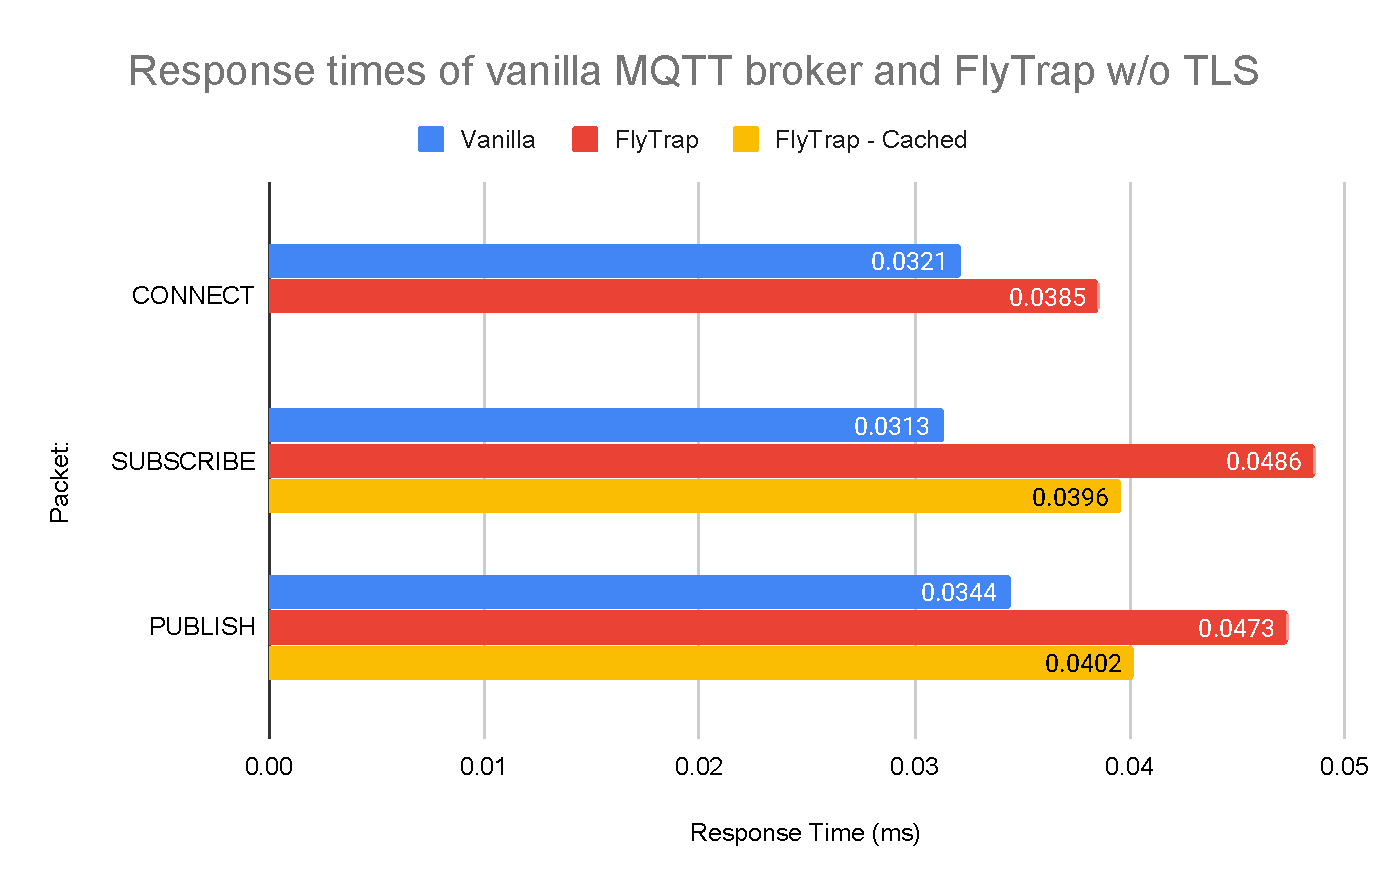
\includegraphics[width=\textwidth]{latency_notls}
    \caption{Response times of most common MQTT requests on plain TCP connection}
    \label{fig:latency_notls}
\end{figure}

In order to deem the results statistically significant, I performed identical tests as in TLS-focused experiment. For each of the tests, the \textit{p-value} was found to be $<0.05$ thus allowing me reject the null hypotheses. Table\ \ref{tab:ttest-notls} shows the specific values of performed statistical tests.

\begin{table}[h]
\centering
\begin{tabular}{|l|l|l|l|}
\hline
\textbf{\#} & \textbf{Test Data}                       & \textbf{Performed Test} & \textbf{p-value}                      \\ \hline
1           & CONNECT: Vanilla vs FlyTrap              & Two Tailed T-Test       & $8.60*10^{-20}$                    \\ \hline
2           & SUBSCRIBE: Vanilla vs FlyTrap vs Cached & Kruskal-Wallis          & $<<< 0.001$ \\ \hline
3           & PUBLISH: Vanilla vs FlyTrap vs Cached & Kruskal-Wallis          & $<<< 0.001$ \\ \hline
\end{tabular}
\caption{Outcome of statistical tests on each the MQTT packets considered on plain TCP connection}
\label{tab:ttest-notls}
\end{table}


\section{Scalability Evaluation}
To perform this test, 100/1000/10000 concurrent clients will be dispatched to PUBLISH a single message, with identical size across all tests, through FlyTrap with TLS enabled. Every client will be dispatched at the same time, as a separate process, thus ensuring that they do not interfere with each other. Each will be identifying with a different Public Key, forcing FlyTrap to perform authentication flow. Then, time when PUBACK has been received will be captured and saved.

\begin{figure}[h]
    \centering
    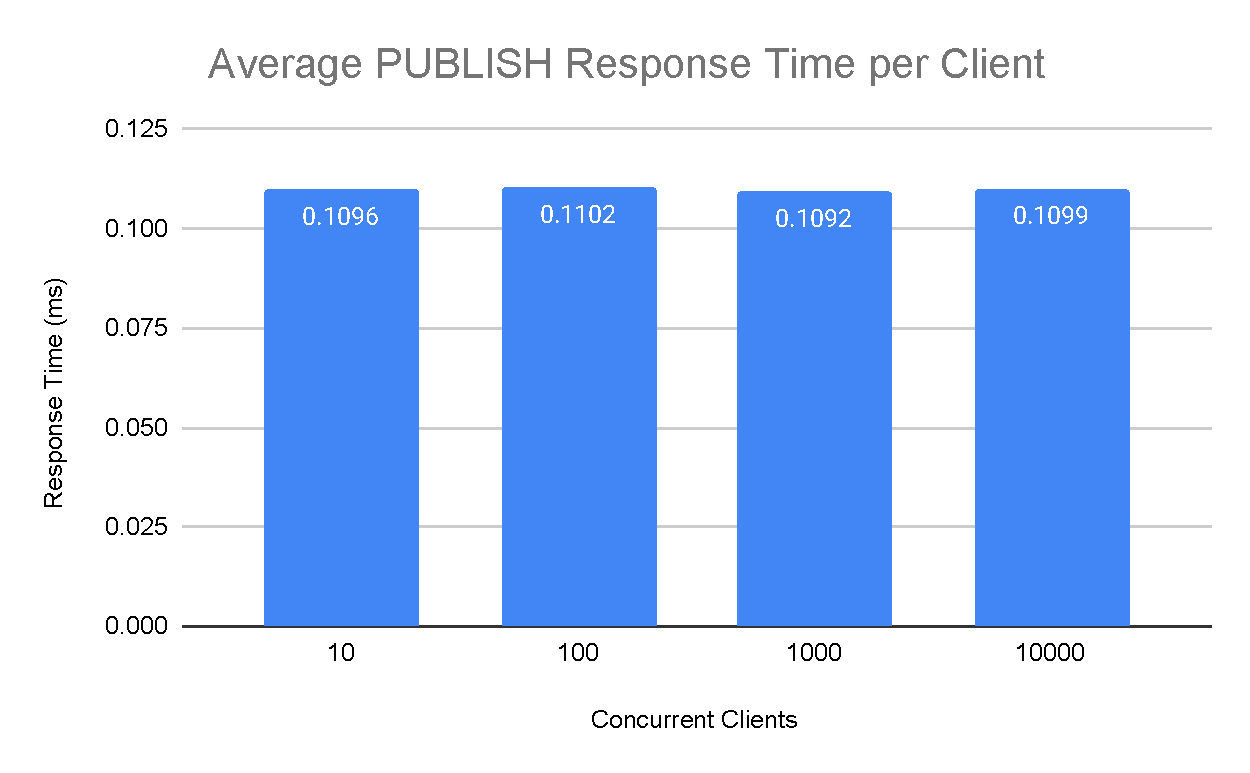
\includegraphics[width=0.8\textwidth]{scale}
    \caption{Average response times with regards to number of concurrent clients}
    \label{fig:scale}
\end{figure}
See figure \ref{fig:scale} with the outcome. We can see that the response time remains constant across a different number of concurrent clients, with less than $1\%$ change between tests.

\section{Cost Evaluation}
As mentioned, Proof-of-Authority networks do not have any currency involved and thus there is no reward for mining. But this removes the benefits of transparency and publicity of the data. On the other hand, running it on a public network (a.k.a. Proof-of-Stake), where miners compete to add new blocks to the network, involves fees and payments and it's important to keep this cost to the minimum.

\begin{figure}[h]
    \centering
    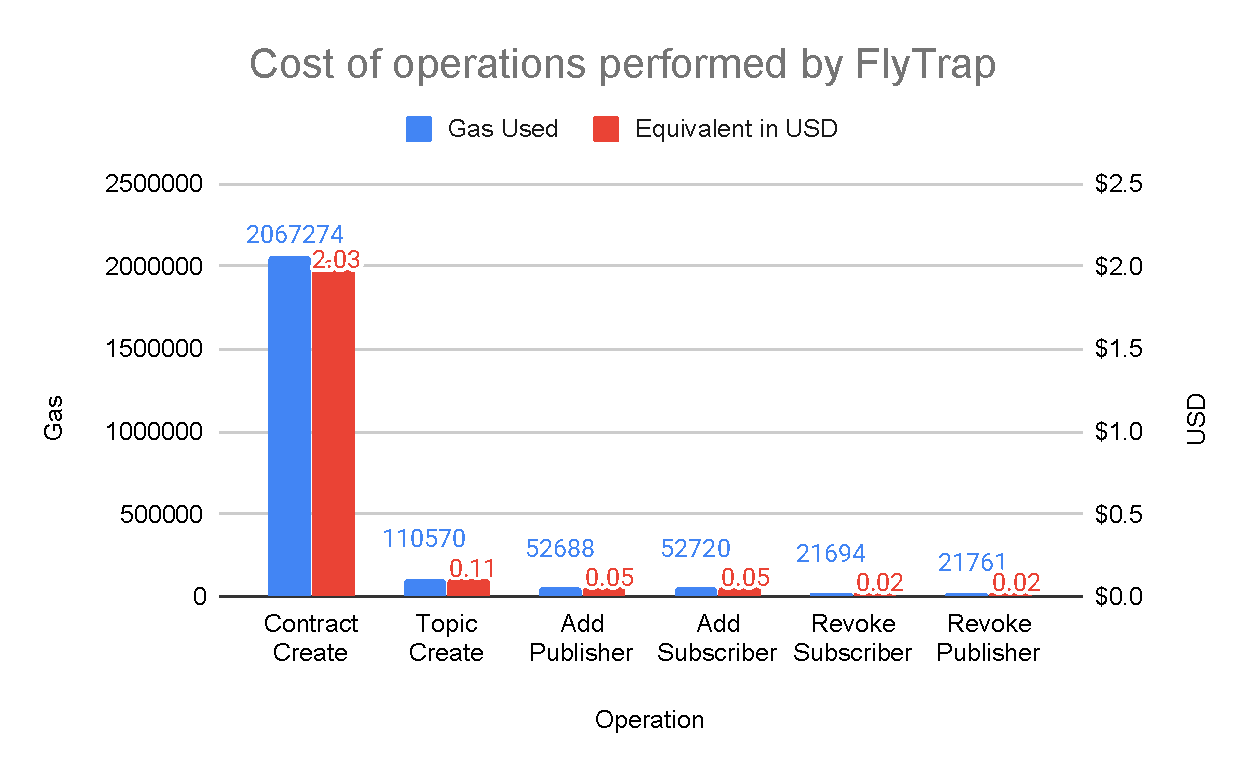
\includegraphics[width=\textwidth]{cost}
    \caption{Cost comparison of various operations on blockchain}
    \label{fig:cost}
\end{figure}

Six operations performed by FlyTrap were executed a hundred times to extract the average costs in gas. To put those numbers into a perspective, I have also included the equivalent value in USD - assuming relations of 1 ETH = \$182.29 and 1 Gas = 0.0000000054 ETH\footnote{Data from https://ethgasstation.info/ and https://cex.io/eth-usd as of 2020-04-18}


\section{Scenarios Evaluation}
In the last test for the evaluation we will be looking at verifying whether the produced software meets the defined requirements in chapter 3. This will focus mostly on a walk-through each of the scenarios, demonstrating how the implemented features satisfy the business need defined in the user story.

Scenario \#5 has been omitted, as the security aspect will be apparent through the remaining tests.
\subsection{Setup}
Each of those scenarios will share common setup steps, which will setup the initial network and proxy. I am going to walk through those steps here - which then can be assumed to be executed prior to any of the subsequent scenarios.
\paragraph{Step 1} - configure your blockchain. For the sake of this experiment, I'm going to use Ganache, which will start a test network, with accounts that have 100 ETH pre-filled currency. Once started, you should obtain a window similar to figure \ref{fig:ganache}.
\paragraph{Step 2} - set endpoint for your blockchain node (Ganache default) and create a new contract for FlyTrap.
\begin{lstlisting}[language=bash]
$ export BLOCKCHAIN_ADDRESS="http://localhost:7545"
$ go run cmd/blockchain/main.go -new -contract=""
2020/04/18 20:28:44 Generated new contract, address is:
0xD0BaD0f1fC6D627E1e6fcE6020De9BbA2507498f
\end{lstlisting}
\paragraph{Step 3} - set contract as environmental variable, add new topic and add publishers/subscribers.
\begin{lstlisting}[language=bash,breaklines=true]
$ export BLOCKCHAIN_CLIENT="0xD0BaD0f1fC6D627E1e6fcE6020De9BbA2507498f"
$ go run cmd/blockchain/main.go -new_topic "creating test topic" -topic "TopicName"
$ go run cmd/blockchain/main.go -topic "TopicName" -client "<client_pubkey>" -pub "adding test publisher"
$ go run cmd/blockchain/main.go -topic "TopicName" -client "<client_pubkey>" -sub "adding test subscriber"
\end{lstlisting}
\paragraph{Step 4} - start web server. Now you should be able to access the website under localhost:8081.
\begin{lstlisting}[language=bash,breaklines=true]
$ go run webapp/main.go
\end{lstlisting}
\paragraph{Step 5} - finally, we are ready to start our FlyTrap proxy. The command will assume TLS as default, with summary reports generated every hour, connection to test mosquitto broker and starts accepting connections under port 8888.
\begin{lstlisting}[language=bash,breaklines=true]
$ go run cmd/flytrap/main.go -b-freq=1h
2020/04/18 21:04:15 Now accepting connections under :8888
\end{lstlisting}
\subsection{Scenario \#1}
For this scenario, we are looking to restrict access to a specific topic, only to people connecting from country which has been permitted. To do so, we will need to slightly modify step 2 from the setup process adding an extra `country' flag to the command, as follows:
\begin{lstlisting}[language=bash,breaklines=true]
$ export BLOCKCHAIN_CLIENT="0xD0BaD0f1fC6D627E1e6fcE6020De9BbA2507498f"
$ go run cmd/blockchain/main.go -new_topic "creating test topic" -topic "RestrictedTopic" -country="GB"
\end{lstlisting}
From now on, only people connecting from British IPs will be allowed, everyone else will be presented with the following message:
\begin{lstlisting}[language=bash,breaklines=true]
$ go run client.go -pub=20 -tls=false -priv="privkey1.asc"
2020/04/18 21:04:17 Using cached signature & public key
2020/04/18 21:04:17 Publishing message: Here Be Dragons #0
panic: error publishing: The PUBLISH is not authorized.
\end{lstlisting}
\subsection{Scenario \#2}
This scenario requires us to determine who access the requested resource on the specific day, so we can determine the scope of the leak. Once the steps in the setup have been completed (in particular, we are about `freq' option) and the leak happens, we are ready to inspect the website.

\begin{figure}[h]
    \centering
    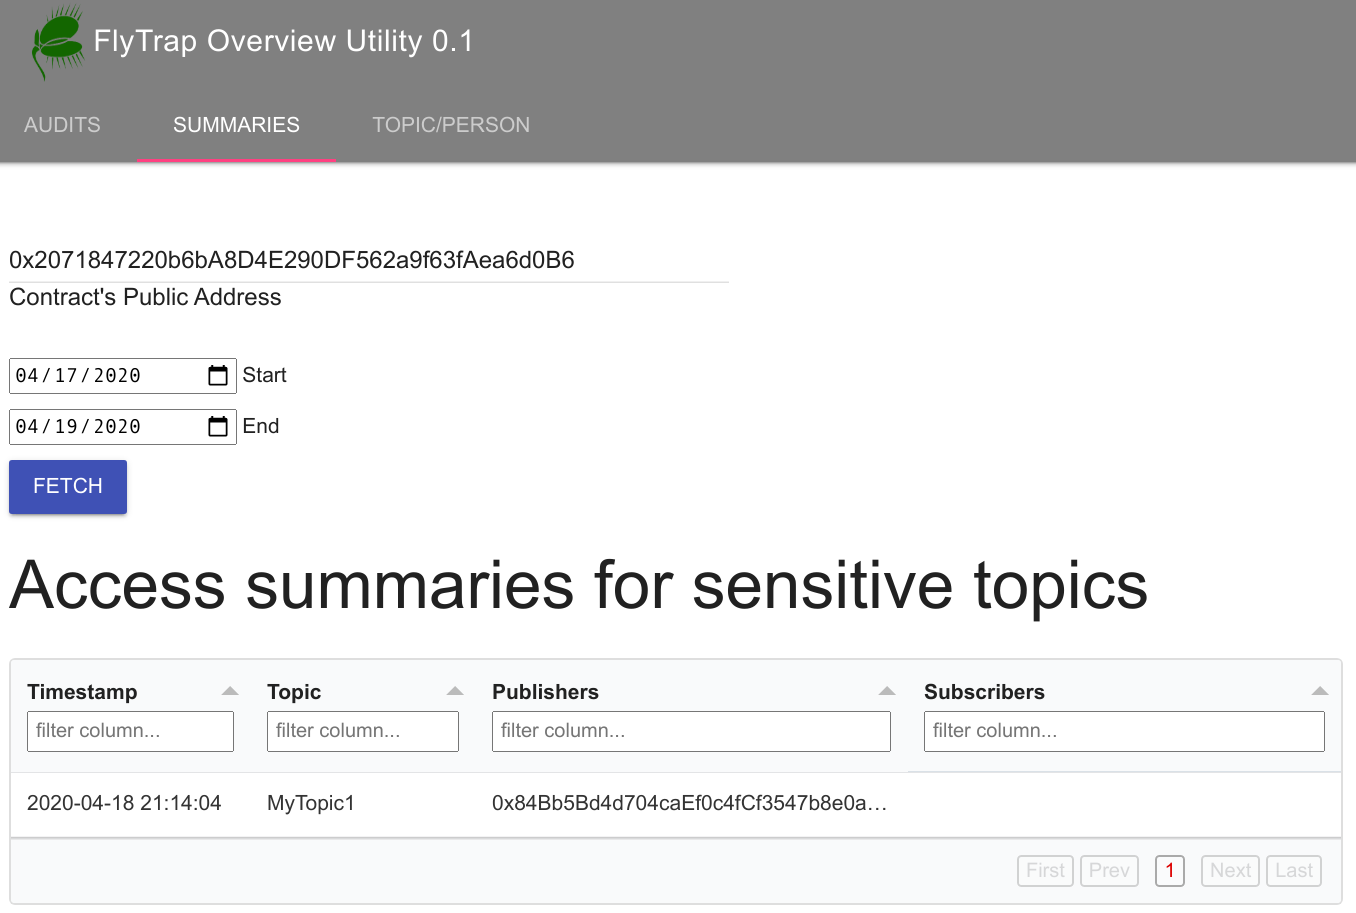
\includegraphics[width=0.9\textwidth]{scenario2}
    \caption{Sensitive topics report}
    \label{fig:scenario2}
\end{figure}
Figure \ref{fig:scenario2} shows how the website would look like upon inspecting the access summaries. We can see that on April 18th in the evening, topic `MyTopic1' was accessed by a single person with the shown public key. Now, we are able to trace the leakage down to a single person and verify whether their credentials were compromised to further assess the damages.
\subsection{Scenario \#3}
Here we are just looking at verifying who can access particular resource, as we want to ensure that all systems that could have read relevant data have been wiped. Again, after following setup steps, we can go ahead and inspect "Topic/Person" part of the webapp, which would allow us to see a list of public keys that can access given topic, as per figure \ref{fig:scenario3}. Then, the system administrator would be able to correlate public key with the piece of infrastructure accessing the information and ensure that the access is revoked along with 
\begin{figure}[h]
    \centering
    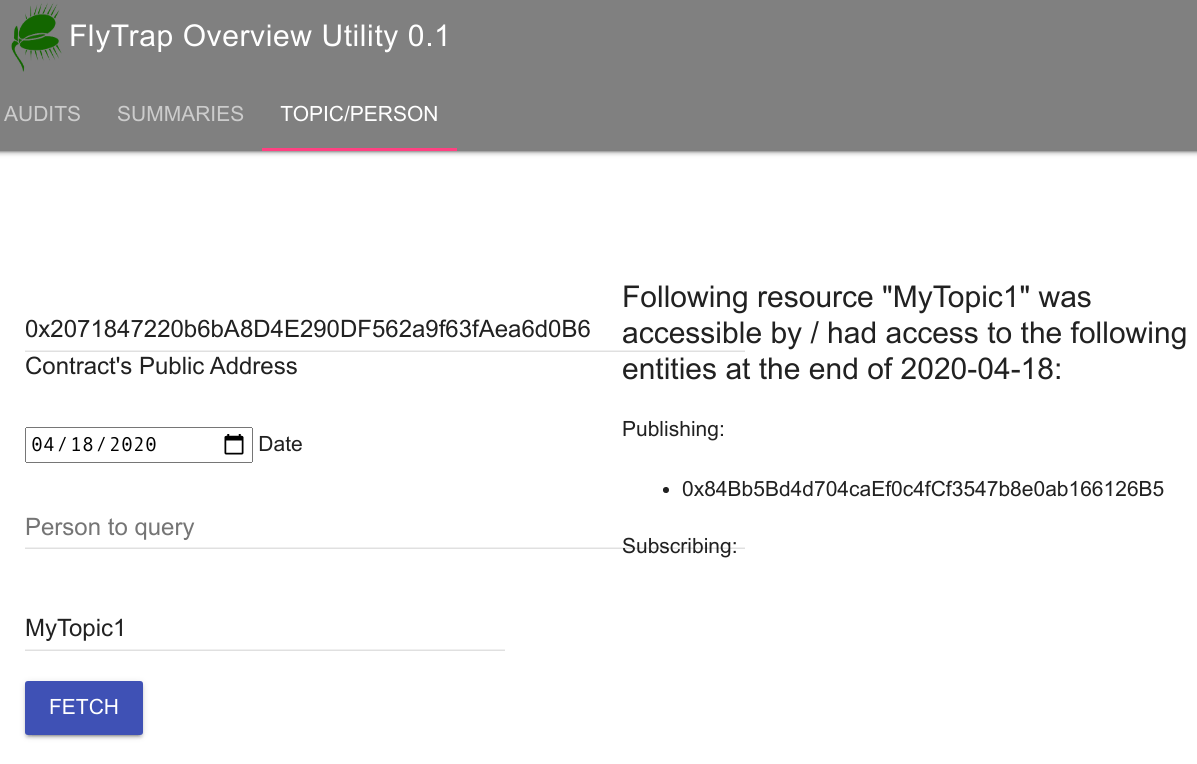
\includegraphics[width=0.9\textwidth]{scenario3}
    \caption{Current Access Control List summary}
    \label{fig:scenario3}
\end{figure}
\section{Results}
\subsection{Latency Evaluation}
The added overhead added by FlyTrap is apparent, reaching even an extra 0.05ms per request. Though, it is interesting to see - looking at ``FlyTrap - Cached'' bar - that caching remediates this problem almost completely, reducing the average response time by up to 37\%, negating the overhead introduced by the first request. We can conclude that FlyTrap would be the most efficient for situations where it is not restarted very often, allowing the cache to grow and in order minimising the impact for clients often connecting to the broker. As expected - we also note longer response time for FlyTrap with TLS enabled. This is most probably caused by the fact that now there need to be two separate TLS sessions established, encrypting/decrypting the data twice.

For FlyTrap with enabled caching functionality, we can notice an average increase of 0.009ms across both plain TCP and TLS when compared with vanilla broker. This is significantly less than specified 500ms in \textbf{NFR1} and thus meets this non-functional requirement and concludes the first research question.

It is also interesting to see that the increased latency is much bigger in TLS connections, when compared to TCP. With TLS, not only we have to deal with an extra overhead of having to contact blockchain to read authentication data, but also perform TLS encryption/decryption twice - first time when communicating with the client and the second time when communicating with the broker.
\subsection{Scalability Evaluation}
On the tested machine, the response times remained constant, indicating that the proxy is capable of handling many concurrent clients without significant impact on performance. If desired, multiple FlyTrap instances can also be deployed across many machines - each pointing to the same broker, further enhacing the response times. This concludes the second research question.

It is important to note that FlyTrap will have an overall limit of maximum allowed concurrent connections of 65535 (equal to $2^{16}$) This is enforced by two limitations. First, MQTT Protocol can only accept Client IDs of at most $2^{16}$ characters long, so naturally it won't be able to proxy more connections than that, since Broker would staright up refuse them. Secondly, FlyTrap operates on linux TCP ports. And again, allowed port range only goes up to 65535. Where the latter problem could be fixed with WebSockets (discussed in the next chapter), the former would still remain a limitation.
\subsection{Cost Evaluation}
For the cost evaluation, the most expensive operation would be creation of the new contract, coming down to \$2.03. Contract contains the bare-bone definition of structures used by FlyTrap, so high price was expected. Though, this only needs to be performed once - the contract can be reused for as many topics as it is necessary. The remaining operations (which would be also performed more often), have their prices much lower. A company looking to create 10 topics with 100 publishers would be looking at an investment of $10 * \$0.11 + 100 * \$0.05 = \$6.1$. This scales linearly and cost remains the same, regardless the current size of the contract and amount of pre-existing topics/publishers/subscribers.

Blockchain offers a solution with 100\% uptime - and at the same time allowing for potential monetisation of accessing the data. The average cost is significantly higher, when compared to centralised solutions, such as SQL server hosted in cloud - but it lacks the benefits of a distributed ledger. Ultimately, all pros and cons would need to be considered before making a decision to utilise Ethereum as a data layer.
\subsection{Scenario Evaluation}
By walking through each of the scenarios, I was able to prove that the software fulfills the business need specified at the beginning of this paper. Scenario's \#4 use-case has been shown to be satisfied through the previous examples, as bare security benefit is considered. For the Scenario \#5, please refer to the User Manual for an explanation on how to set a cost on addining new publishers or subscribers.

% \chapter{Conclusion, Discussion and Future Work\label{chap:discussion}}
In this chapter, I conclude the work conducted in this paper, reflect on the results and suggest the next steps for the designed framework. I also overview my achievements, slowdowns and difficulties found.

\section{Summary}
In this dissertation, I have introduced a novel method of authenticating clients connecting to arbitrary MQTT Brokers through a middleware framework storing persistent information on Ethereum blockchain, allowing for higher transparency and availability. I have started by providing a motivation for the project, bringing up that standard MQTT protocol offers only limited authentication methods, with no option to log audit trails. Recent legislature requiring data administrators to adhere to a specific set of rules dictating how the data should be stored, maintained and erased if requested was also discussed.

As the project involved a lot of sophisticated software such as MQTT or Blockchain, a thorough background chapter was included in order to allow the reader to better understand the concepts and decisions taken throughout this thesis. An overview of related papers has also been included to make sure that my efforts were not duplicating any similar research.

Before discussing the design of the framework, I explored and listed requirements for the project formulated as user stories, scenarios and list of functional and nonfunctional requirements. Next, I proceeded with presenting a proposed architecture for FlyTrap, splitting it into four, independent modules: proxy, client, web app and blockchain - each capable of working on its own. I've discussed the data model stored on the blockchain and how access to sensitive topics is continuously logged to allow tracking back entities reading the data.

Then I went on to talk about the implementation details, discussing the workflows that I have been following, my testing strategy and how my development environment looked like. In particular, simulating both MQTT Broker and Blockchain posed a challenge, as both are somewhat sophisticated frameworks often requiring many modules to function correctly.

Finally, I designed experiments aiming to evaluate FlyTrap's feasibility, how severely the performance hit was, whether the software is capable of scaling up as the number of concurrent clients might go up, cost of operating on Proof-of-Stake blockchain network and reflected to scenarios to determine whether specified requirements have been met. The increased response time through FlyTrap ranged from $18.12\%$ to $62.67\%$ when compared to vanilla broker. FlyTrap was also found to scale effortlessly, with almost no loss as the number of clients increased. Operational cost included a one-off payment of circa \$2.03, with general costs of circa \$0.11 per operation.

Detailed User Manual and Maintenance Manual have also been included as appendices, to outline how to set up your own proxy and how to read the source code created in this project.

\section{Discussion}

\subsection{Proof-of-Stake vs Proof-of-Authority}
When I first introduced the concept of blockchain in this paper, I discussed the differences between proof-of-stake and proof-of-authority consensus algorithms. As a reminder, Proof-of-Stake involves mining rewards for adding new blocks to the chain (thus involves currency) and is currently used for the public Ethereum network, whereas Proof-of-Authority does not involve any rewards and all blocks are verified by a set of ``sealers'' whose job is to verify whether they can be processed or not.

\begin{figure}[h]
    \centering
    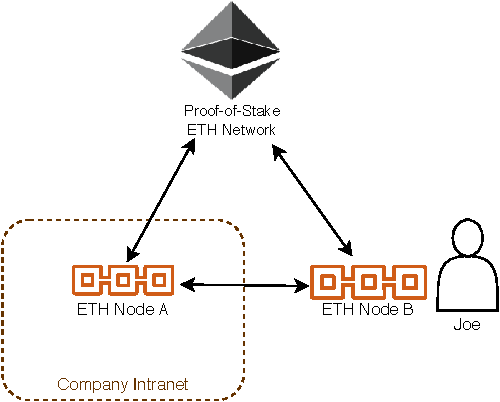
\includegraphics[width=0.7\textwidth]{blockchain_pos}
    \caption{Public Proof-of-Stake network}
    \label{fig:blockchain_pos}
\end{figure}
\begin{figure}[h]
    \centering
    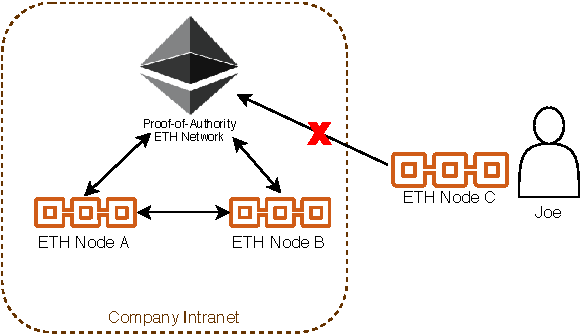
\includegraphics[width=0.75\textwidth]{blockchain_poa}
    \caption{Private Proof-of-Authority network}
    \label{fig:blockchain_poa}
\end{figure}

Figures \ref{fig:blockchain_pos} \& \ref{fig:blockchain_poa} illustrate those differences. In the first example, the company has complete control over its blockchain network, and nobody from the outside can read it or add new blocks. Even though Joe has configured his own node, he will not be able to connect to it. In the second example, the company is connecting to the public node, to which Joe - and anyone else - can also connect to read or submit new blocks.

Let us first look at Proof-of-Stake. This includes all benefits coming from blockchain architecture.  That is, the entire layer is decentralised, meaning that hardware failure will not cause data loss, as every participant will be holding a copy. This ensures a pure 100\% uptime of the data layer. Moreover, all transactions are transparent and immutable. Nobody can deny submitting it or alter the past by removing some blocks from the chain (which is not even possible, to begin with) - perhaps this would be the most beneficial for the authorities and law enforcement organisations, which no longer have to trust data provided by the company, as they can host their own node and read stored data.

\subsection{Comparison with State-of-the-Art}
Both IoT and Blockchain are still developing technologies, which only recently gained traction in the industry. The lack of a similar solution forced me to look beyond the original scope of the project and investigate papers which were also combining those two concepts. Because of that, state-of-the-art comparison involves only the un-changed MQTT Broker. I was satisfied to see only a minor increase, while providing the extra authentication and accountability capabilities.
\section{Reflection}
This section will reflect back on the challenges that I faced when working on this project. I will also outline things that went exceptionally well and things that did not go as planned.
\subsection{Achievements}
Before deciding to work on this particular topic, I did not know MQTT or blockchain. I only briefly heard about such technologies, but never had a chance to apply them in any of my projects. The majority of time working on this dissertation was spent on background research and learning how to bring up my own Ethereum network, research industry trends and conducting a thorough evaluation to assess my solution.

I am also happy to say that I successfully followed my original project plan, only with minor deviations. At no point I was facing pressure or closing on deadlines, always leaving an extra week or two as a buffer in case things did not go as expected.

Writing such lengthy documentation was also always a challenge for me, so I am very proud that I was able to stay persistent and finalise this project, gaining valuable research experience.

\subsection{Difficulties \& Lessons Learnt}
When starting to plan this project at the end of the last year, I never anticipated that I would have to conduct it in circumstances of a worldwide lockdown. I have to admit, working on my project entirely remotely has been a big challenge which made me appreciate face-to-face teaching \& guidance even more. As much as my online meetings were going smoothly and without problems, I started to miss the whiteboarding in my supervisor's office - which was invaluable during brainstorming.

As I planned my risk management when writing the project plan, I didn't take global pandemic into account - and I don't think that anyone did. With remote work, I lost the benefit of networking with my peers and discussing our ideas, which provided an immense help before. We were able to overcome this challenge by organising a weekly remote meetup through videoconferencing to carry on, as we knew that the help that we can offer each other is invaluable.

I also learned to always ask for help if faced with a roadblock for an extended time. For example, at one point, I encountered a problem where my software was no longer capable of handling concurrent clients. I spent roughly 2 days dissecting my code line by line, to determine the root cause and eventually pinpointed it to the fact that the Client ID field needs to be unique for the broker to respond. When discussed it with one of my co-supervisors, I learned that he also faced a similar problem in the past and also got stuck for a couple of days. If I approached him earlier, I could have saved those two days.

Several technical challenges also came up, that I either had to omit from the final implementation or think about a workaround. One of the examples being the sheer cost of operating applications on a distributed platform. It is incredibly easy to start exhausting the resources (and thus bumping the price) exponentially, so I had to think about limiting potential writes to a minimum. That's how the caching and crafting data models came to life, as I started to become concious of available resources. Another example is TLS, which almost doubled the response times. I learned that sometimes it might be more desirable to decide against TLS in favour of plain TCP in order to have a more responsive solution.

\section{Future Work}
This section will outline the possible future for FlyTrap and how it could be brought forward with further enhancements to the provided security.
\subsection{Testing TLS}
Following up from the evaluation chapter, we observed a significantly increased performance loss when proxying TLS connections from Client towards FlyTrap and then from FlyTrap to MQTT Broker. Further testing could be needed to determine whether the impact is more significant on \mbox{Client<->FlyTrap} or FlyTrap<->Broker side and provide appropriate guidance on how to provide the best possible performance.

For example, for situations where both FlyTrap and MQTT Broker are located on the same network, it would be wasteful to encrypt packets flowing between FlyTrap and Broker, as man-in-the-middle attacks would not be possible, since all traffic occurs on loopback network device\footnote{Also known as localhost, i.e. inter-process communication through TCP.}. It would be interesting to see whether enabling TLS only on the first part of the journey provides any significant gains.

Furthermore, alternative methods of encrypting TCP packets should be explored. This project uses the standard TLS session with all settings left at default, so tests involving different cypher suites and different key-exchange algorithms would be beneficial.
\subsection{WebSockets}
The most recent versions of popular MQTT Brokers (such as Mosquitto) introduced support for WebSockets - with many of the testing online brokers already offering support, e.g. HiveMQ WebSocket-based broker can be accessed under broker.hivemq.com:8000. WebSocket \cite{fette2011websocket} is built on top of HTTP layer, meaning that all traffic flows through a single port. It is no longer necessary to utilise multiple ports to send concurrent messages.

\begin{figure}[h]
    \centering
    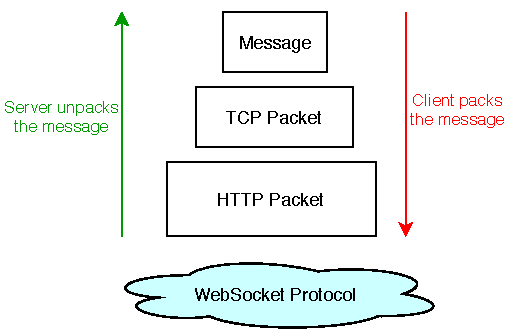
\includegraphics[width=0.7\textwidth]{websockets}
    \caption{Overview of WebSocket protocol}
    \label{fig:websockets}
\end{figure}

Figure \ref{fig:websockets} demonstrates how messages are encapsulated by the client and then unpacked by the server. The most apparent benefit is the increased number of possible proxy connections. FlyTrap currently is tied to the maximum of 65535, which is the maximum number of ports on Linux. Additionally, many firewalls forbid outgoing and incoming connections from non-standard ports. Whenever a new proxy connection is initiated, FlyTrap opens a new ephemeral port, which could otherwise be blocked.

At the moment, the framework operates solely on the TCP layer, sending raw TCP/TLS packets. By adding support for the WebSocket protocol, the limit of maximum concurrent connections could be increased, and by limiting it to a single port (for example, 80), it could become more accessible to devices behind strict firewalls.
\subsection{Device Authenticity}
FlyTrap currently relies only on authentication through a signature containing the public key, signed by the corresponding private key. While it works perfectly fine for the purposes of this project and provides a reasonable protection barrier from attackers, it does not take into consideration situations where the IoT device containing the private key/signature gets stolen, and its data becomes compromised. At this point, the attacker could calculate their own signatures and start making requests against FlyTrap. IoT devices are often neglected when it comes to physical security - they are often placed in public spaces, where anyone could potentially remove it. Normally, it is not a concern, as they are not targeted due to their low cost, but by containing secret data (and signature / private key could be considered secret), it might cause them to become a target.

This problem fell out of scope for this project, and thus it was not considered when designing the system. To tackle this, one might want to introduce methods of verifying the authenticity of connecting devices. In 2012 Apple filed a patent with the United States Patent and Trademark Office \cite{omernick2012systems} offering a solution for this problem. In the future, ideally, FlyTrap should be enhanced by a similar solution, such that it would be able to identify whether the connecting device is a genuine IoT sensor or an attacker connecting from a laptop.

\section{Conclusion}
Through my work in this project, I have shown how Ethereum and MQTT can be combined to provide an efficient Authentication and Accountability framework for MQTT brokers by utilising decentralised blockchain as a data layer. This solution provides a novel set of features such as brute force attack protection, data access monetisation (by collecting payments in a form of cryptocurrency) or a user-friendly front-end to browse the past transactions in order to answer common GDPR questions. The evaluation also proved that the performance impact is acceptable with regards to the gained features. Due to the complex set of dependencies, it is currently aimed at business that are already using blockchain and MQTT, since for them the setup overhead would be minimal. But with the increasing popularity with decentralisied solutions and IoT, FlyTrap could also help business looking to switch, as all needed components (such as MQTT client, front-end or Blockchain CLI) are provided as part of the solution. FlyTrap also has an exciting collection of future work suggestions, which might make it even more accessible and attractive to the potential customers.

% \include{conclusion}

\appendix
\include{proof}

\bibliography{mybib}

\end{document}
